
Data to background comparison of variables from reconstructed objects after 
applying \PQb jet selection as described in Section~\ref{s:secEvtSel} are shown in 
Figures~\ref{fig:btagPlot1},~\ref{fig:btagPlot2}, and~\ref{fig:btagPlot3} for
\mujets and \ejets channel. There is a good agreement between data and simulated background 
within statistical and systematics uncertainties for all variables except for the \pt (of lepton 
and jets) and \MET. There is a poor agreement between data and background for 
higher values of \pt and \MET. The disagreement in these distributions can be 
fixed by applying the \PQt quark \pt weights. However, the \PQt quark \pt weights do not affect 
the $\mjj$ distribution which is the final observable for this analysis.
Therefore, we do not apply \PQt quark \pt weights. The \mjj distribution after \PQb jet selection
is shown in Figures~\ref{subfig:mjj_muBTag} and \ref{subfig:mjj_eleBTag} for both channels
where we do see a good agreement between data and SM backgrounds.

%After BTagging: Pt_lep, Eta_lep, Pt_jets, 
\begin{figure}
    \centering  
    \subfigure[\pt of muon]{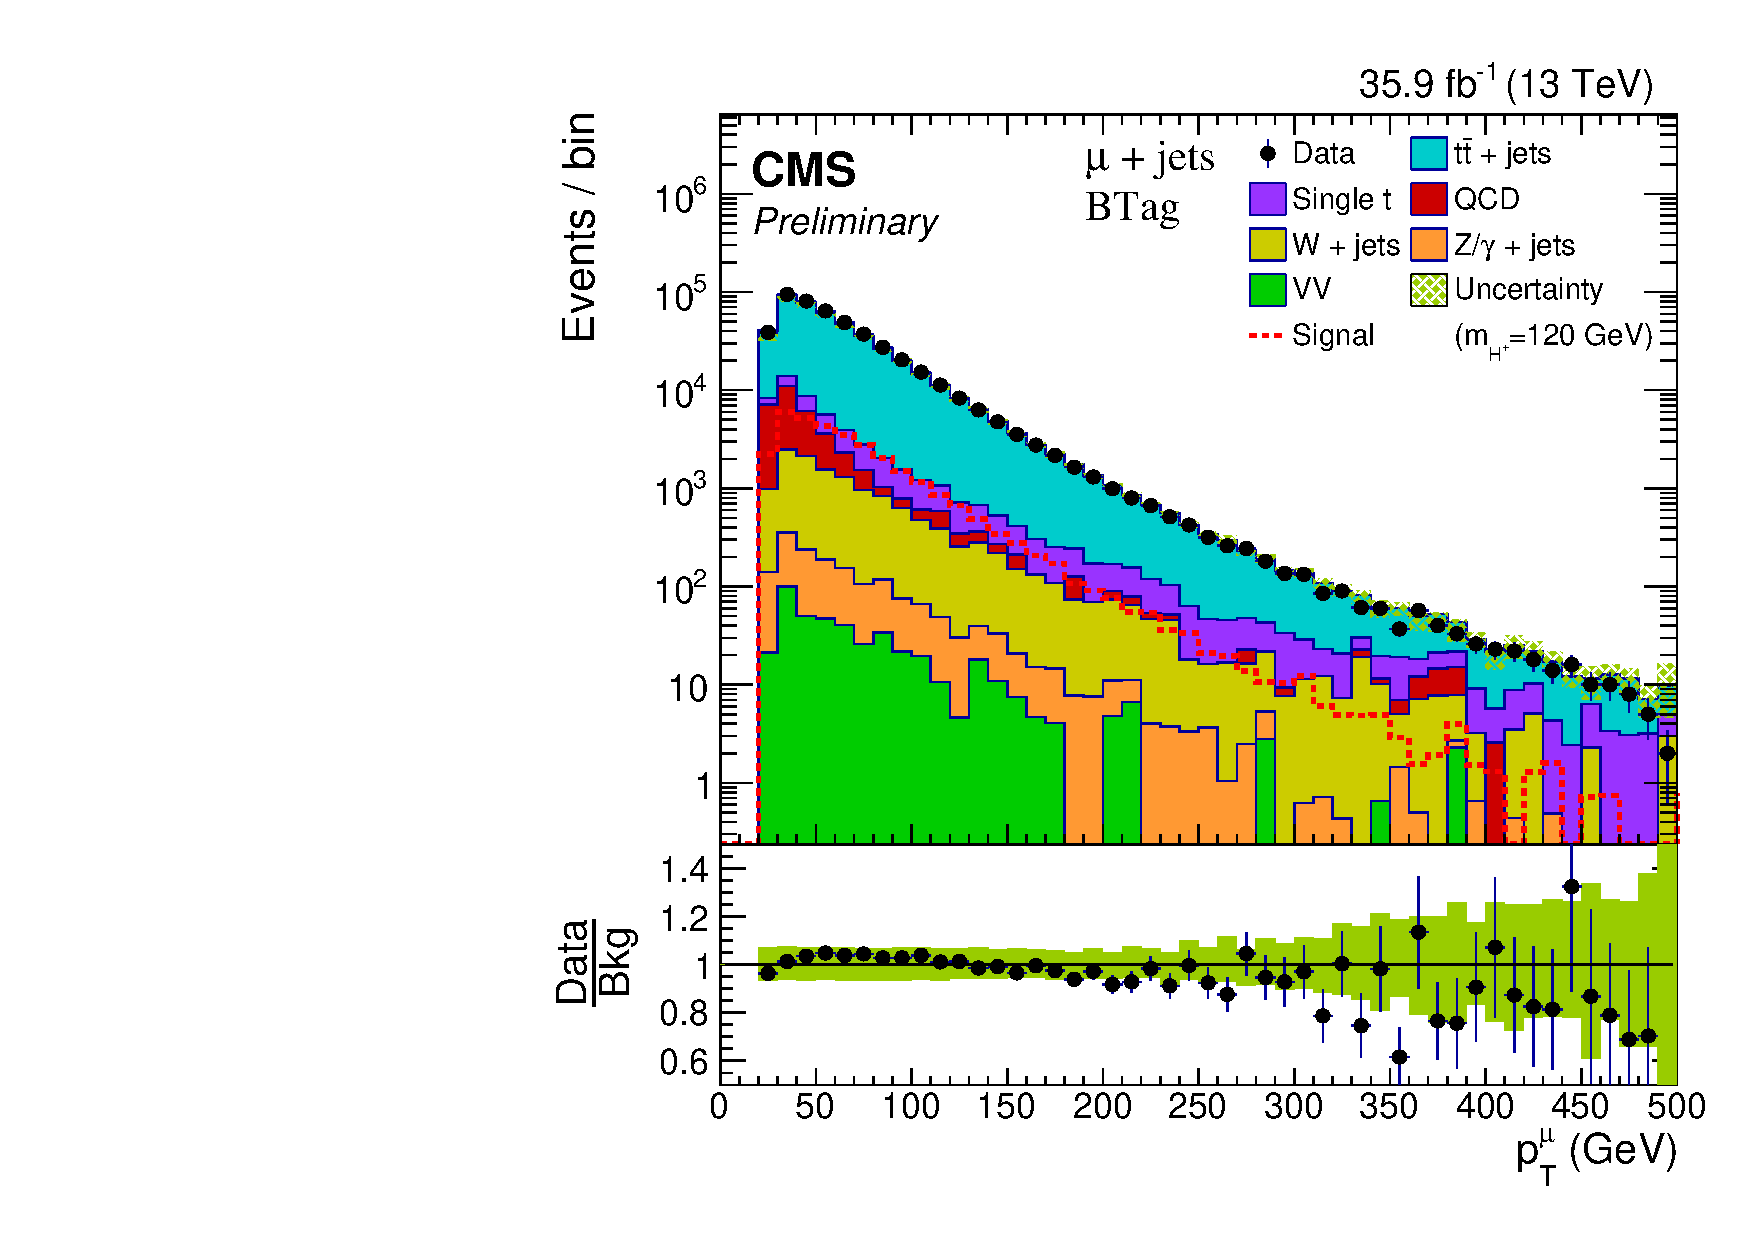
\includegraphics[width=0.40\linewidth]{Image/Muon/BTag/pt_mu_muBTag.pdf}}
    \subfigure[\pt of electron]{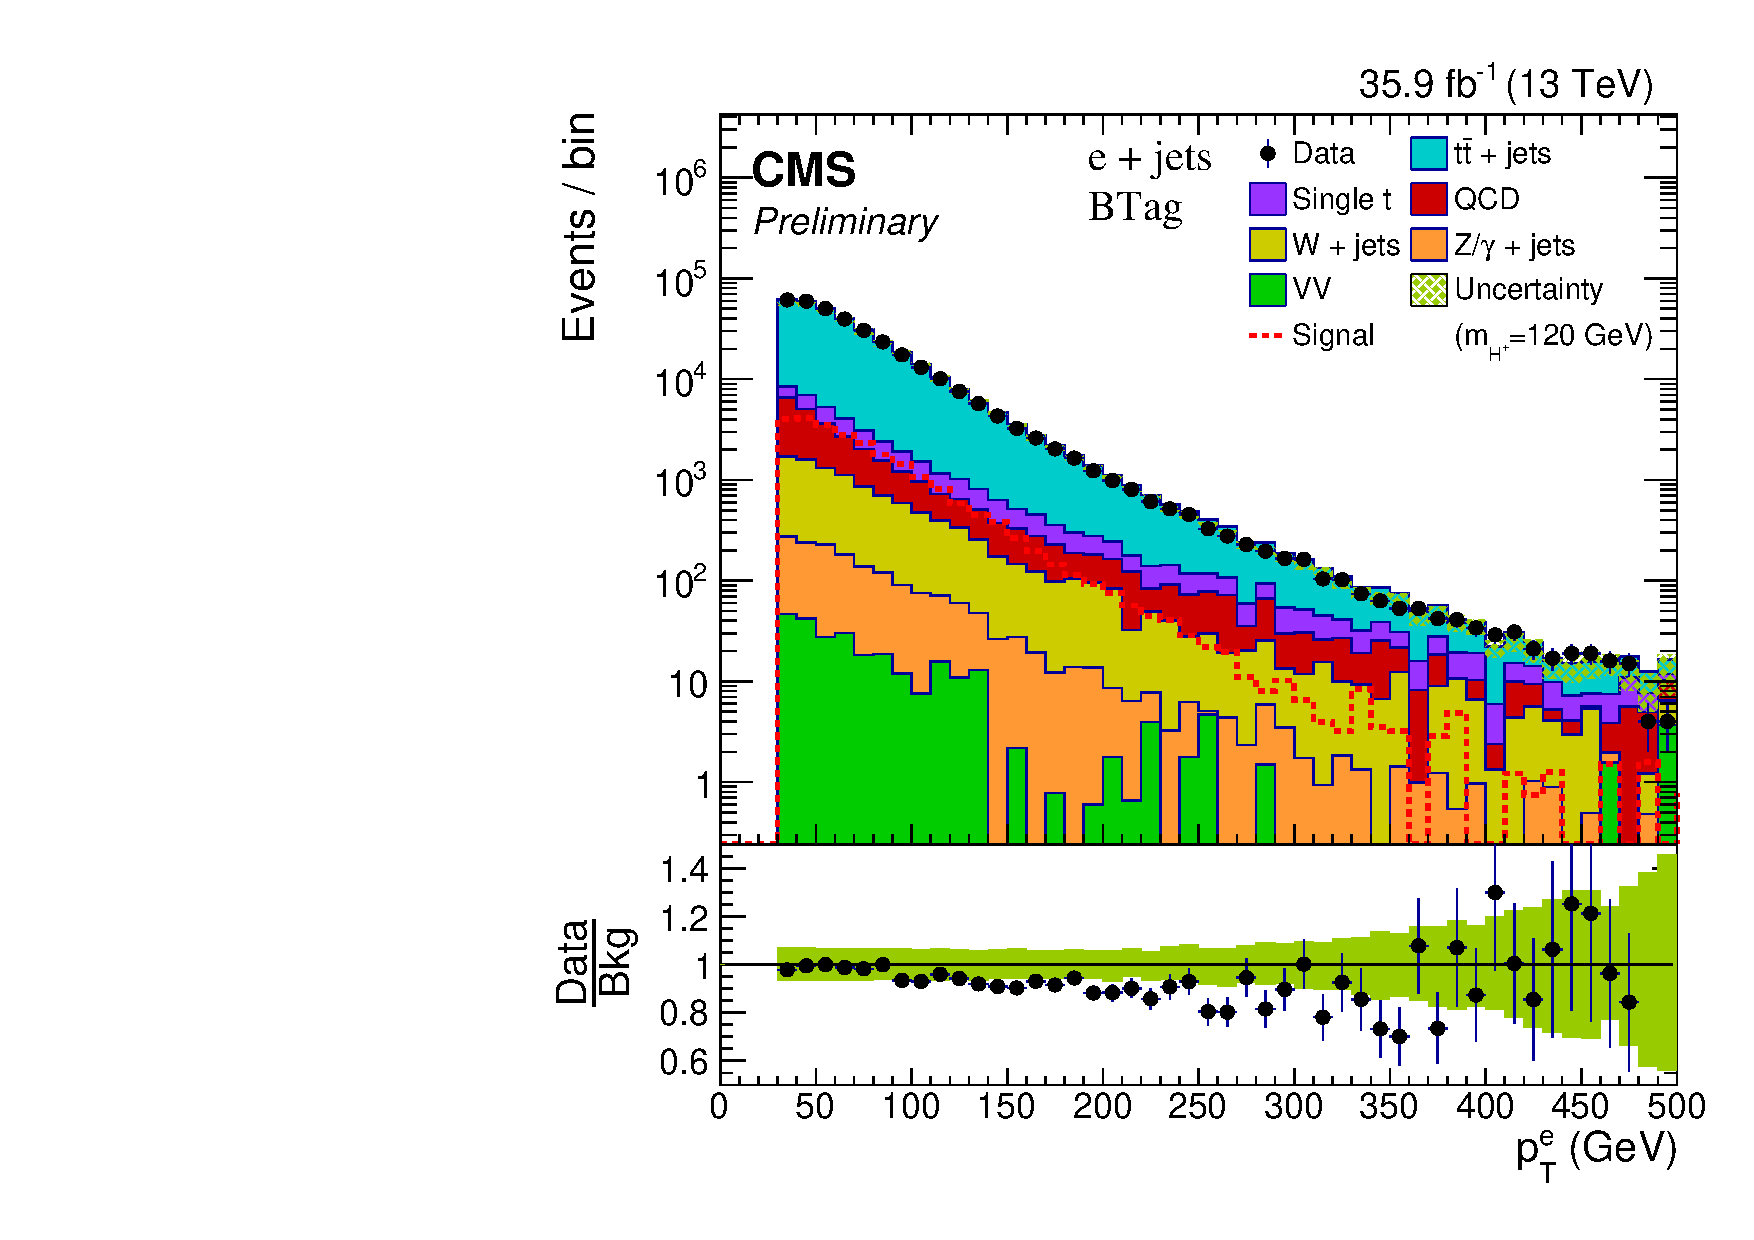
\includegraphics[width=0.40\linewidth]{Image/Electron/BTag/pt_ele_eleBTag.pdf}}
    \vfil
    \subfigure[$\eta$ of muon]{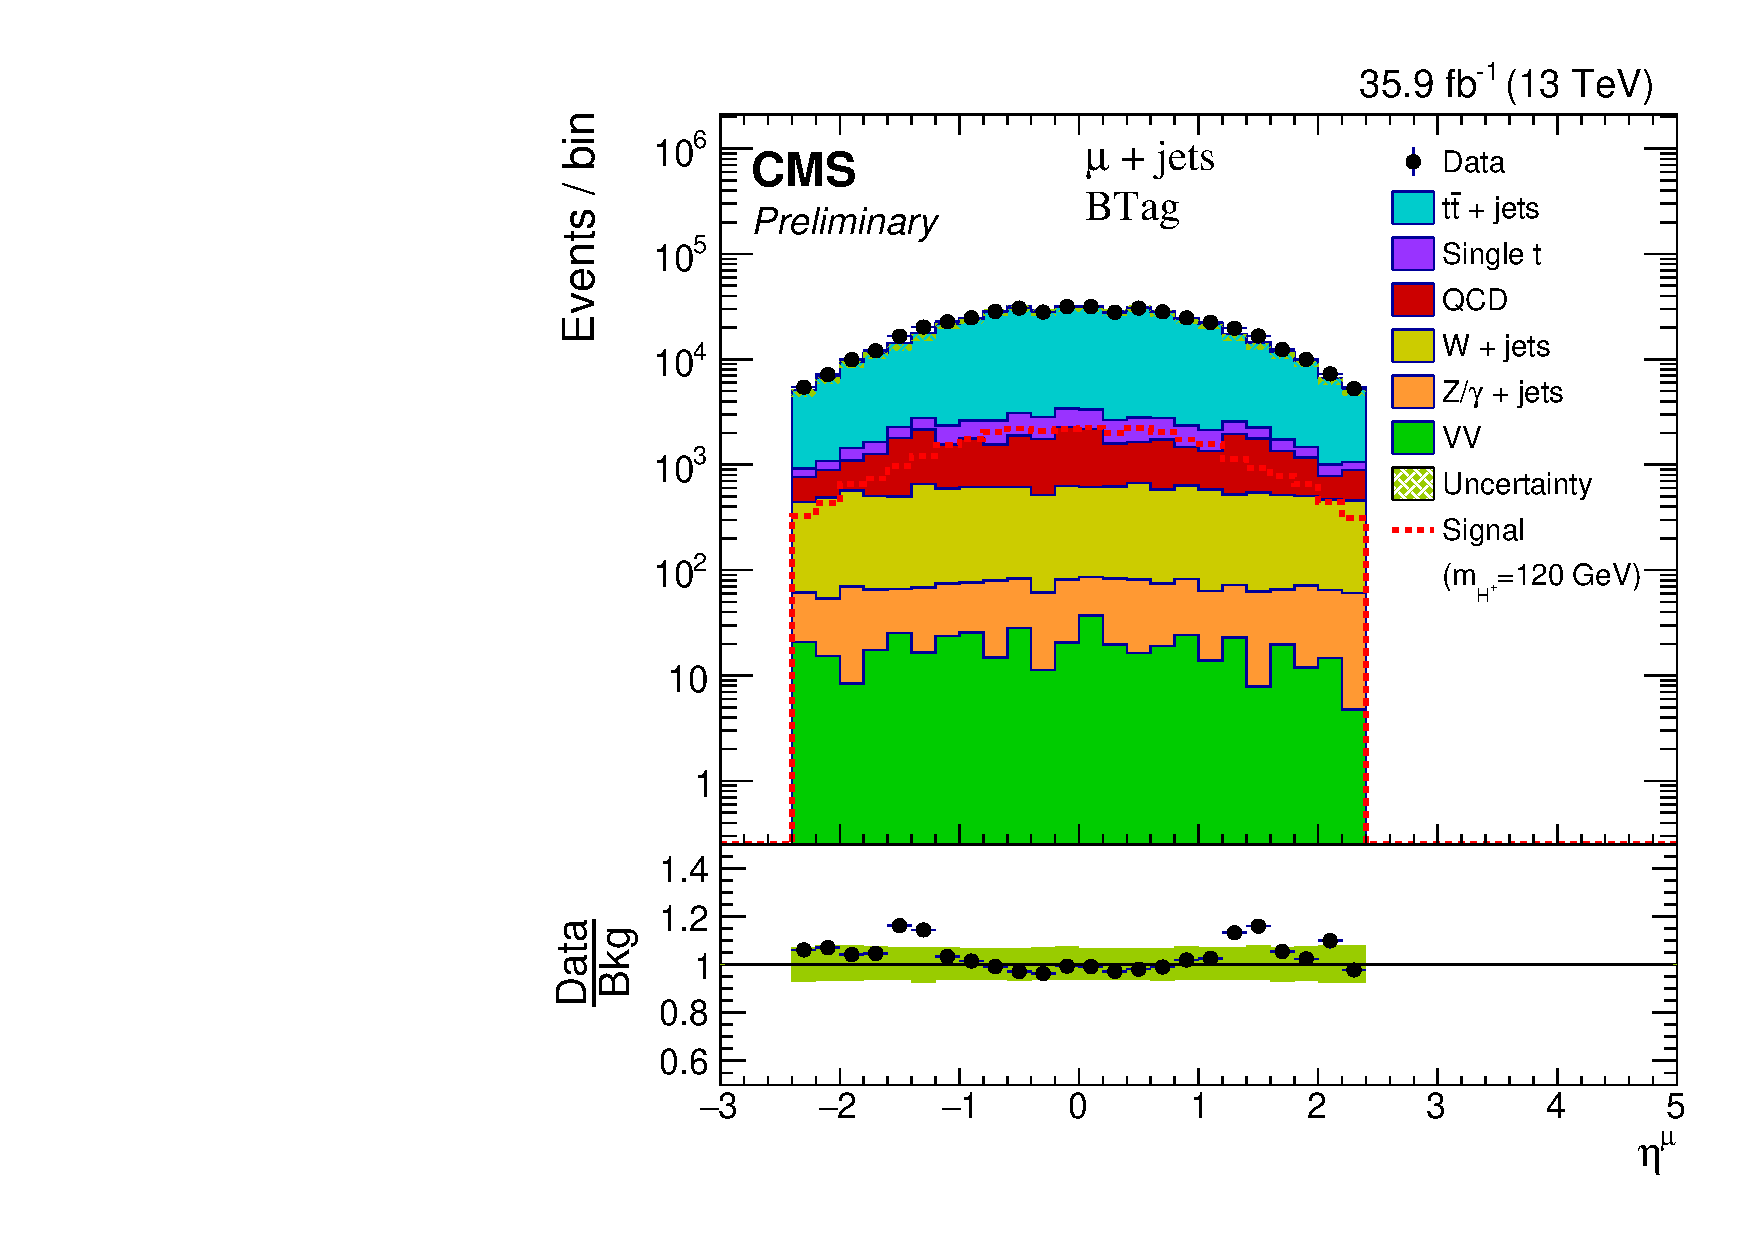
\includegraphics[width=0.40\linewidth]{Image/Muon/BTag/eta_mu_muBTag.pdf}}
    \subfigure[$\eta$ of electron]{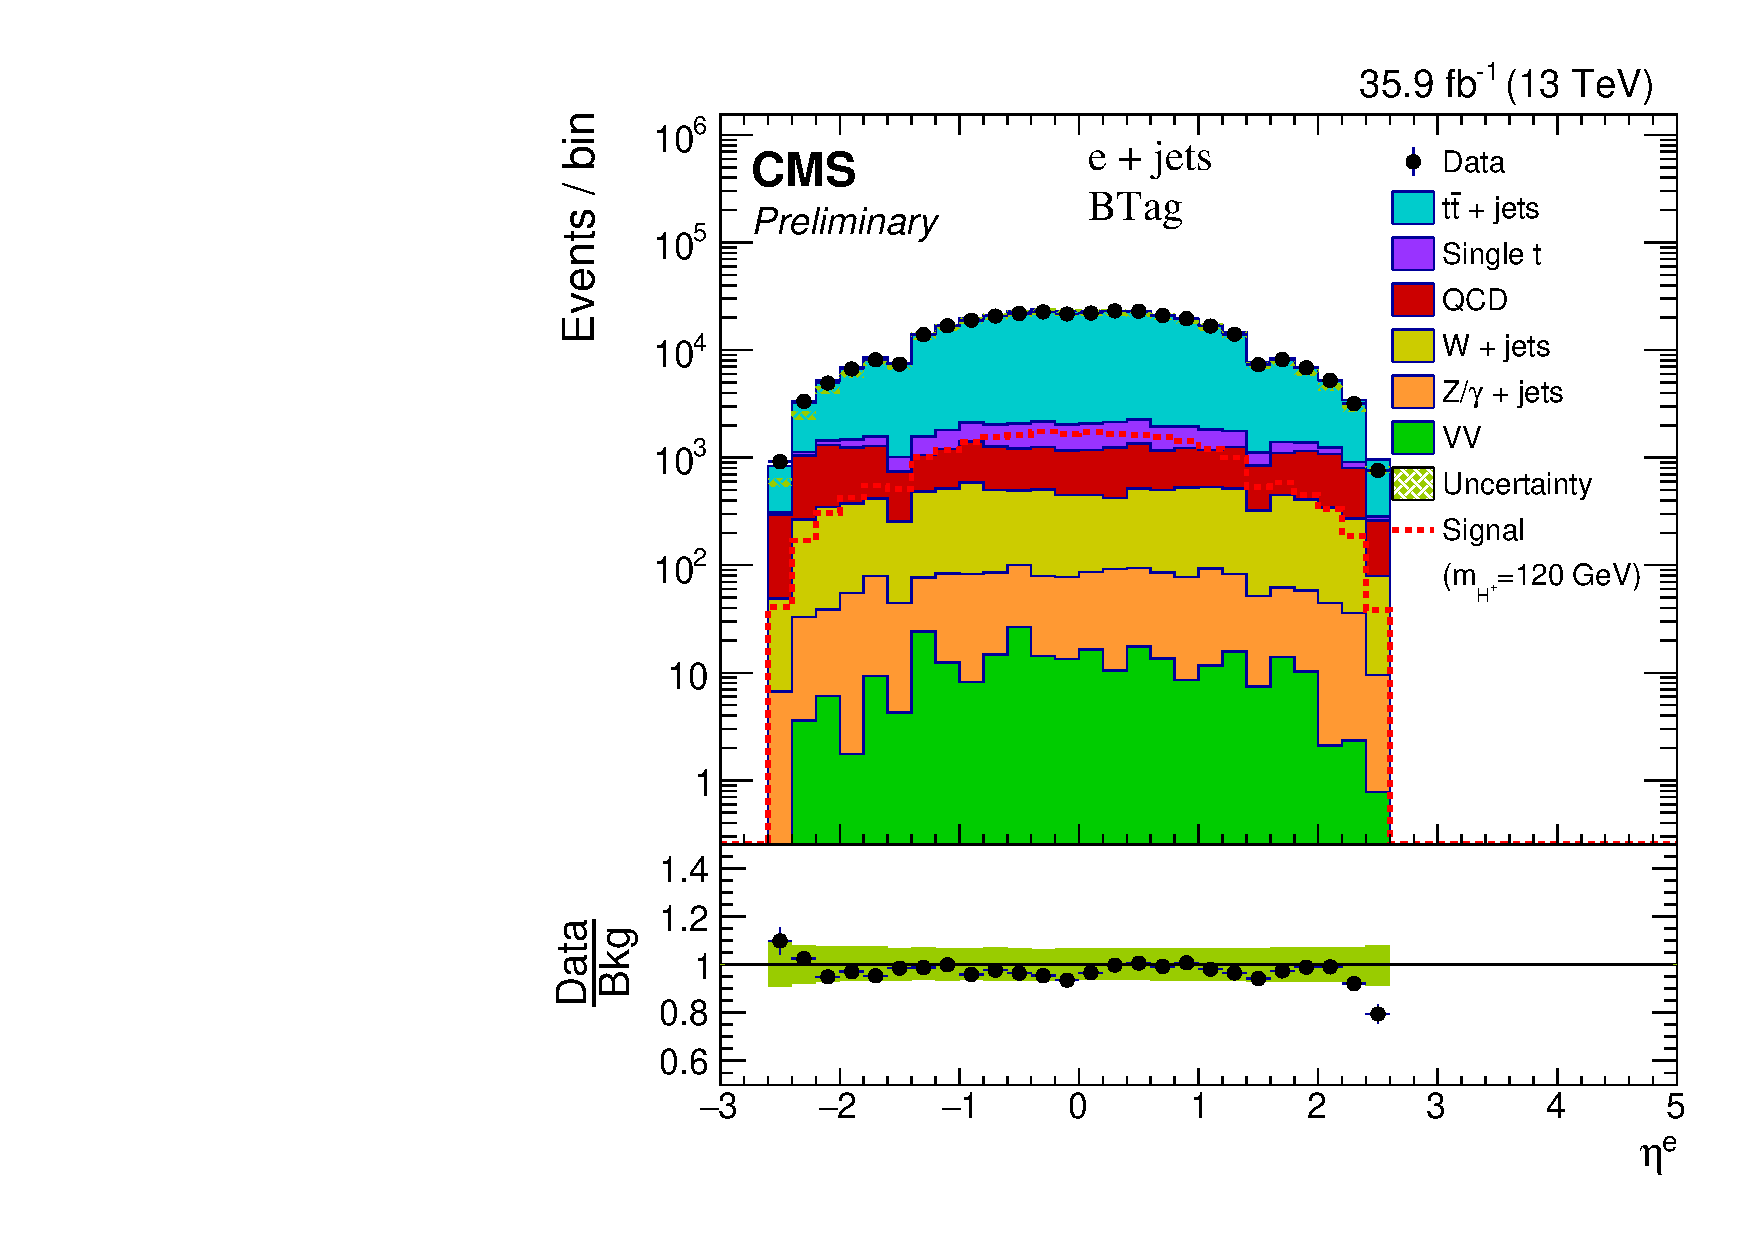
\includegraphics[width=0.40\linewidth]{Image/Electron/BTag/eta_ele_eleBTag.pdf}}
    \vfil
    \subfigure[\pt of jets]{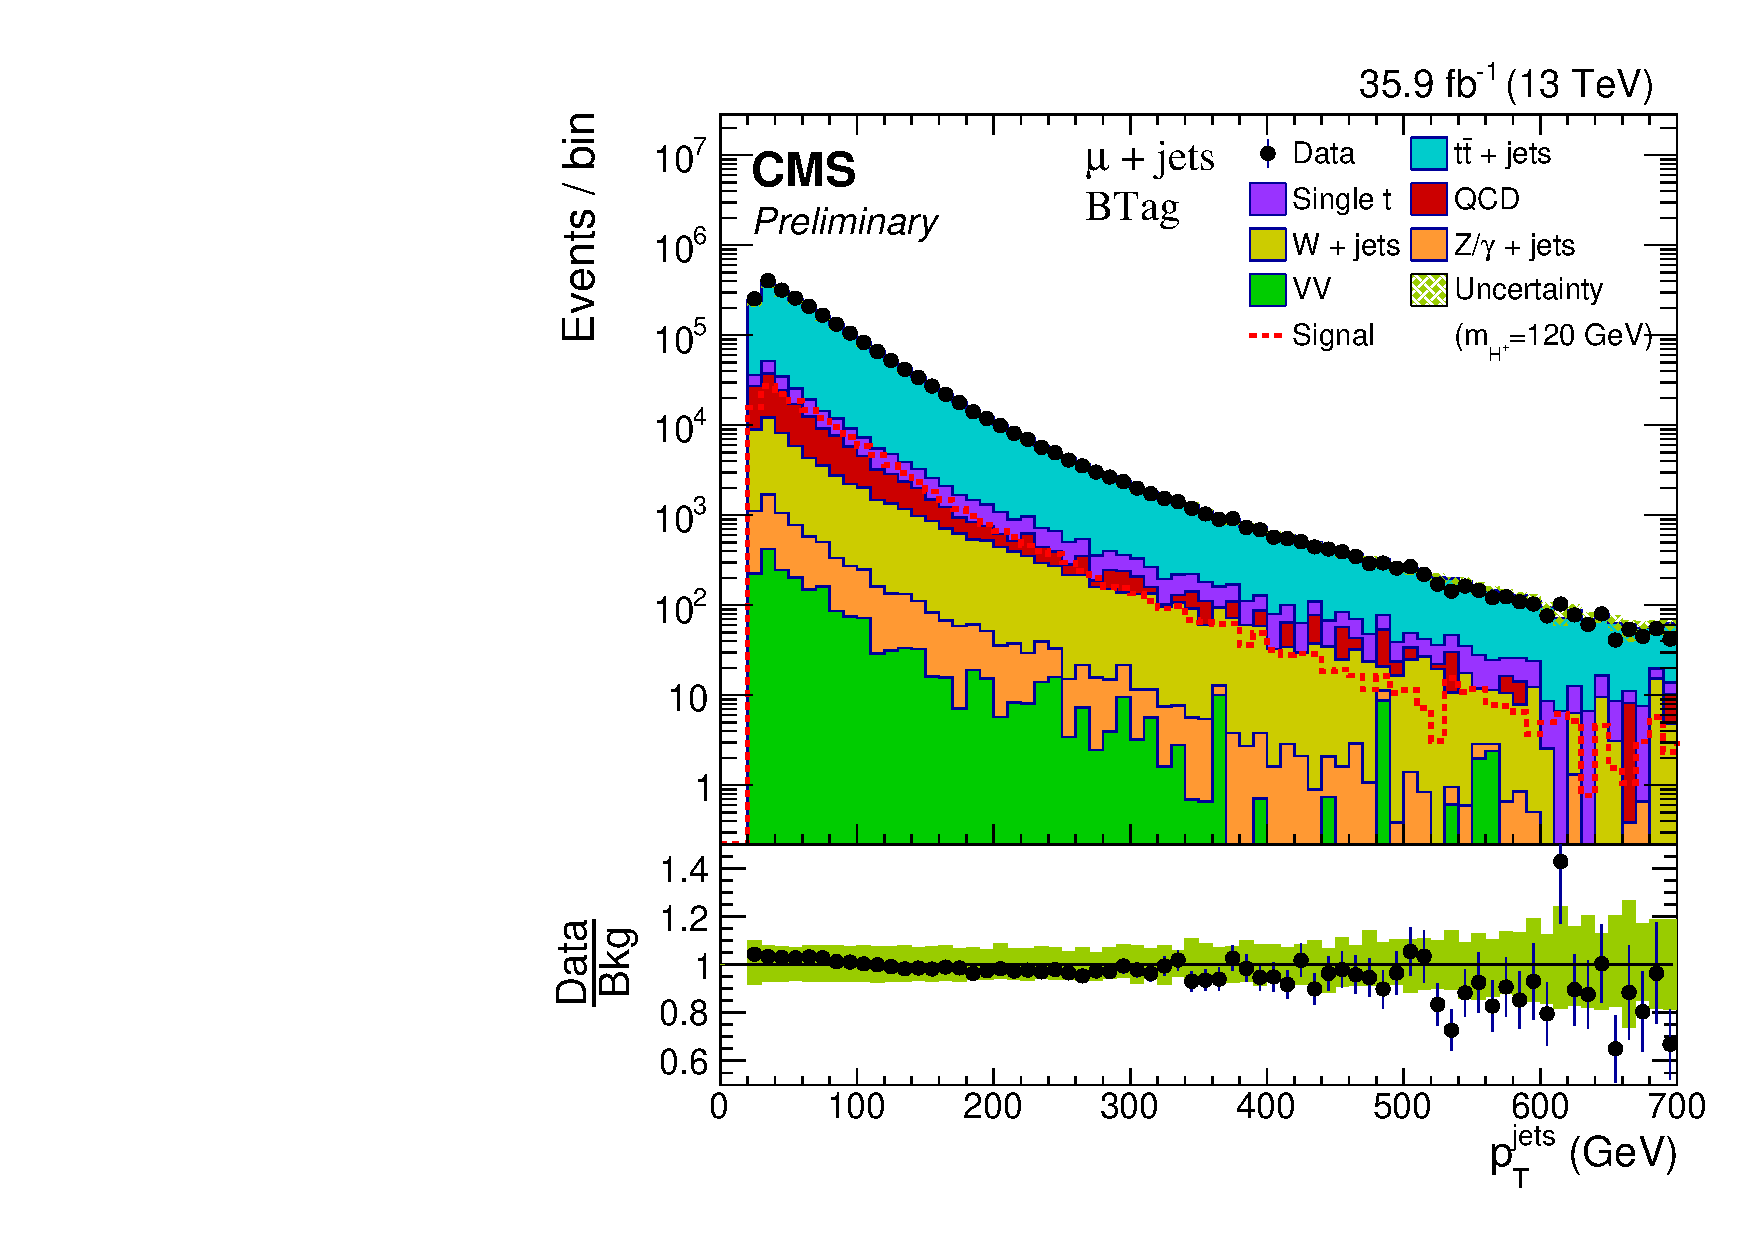
\includegraphics[width=0.40\linewidth]{Image/Muon/BTag/pt_jet_muBTag.pdf}}
    \subfigure[\pt of jets]{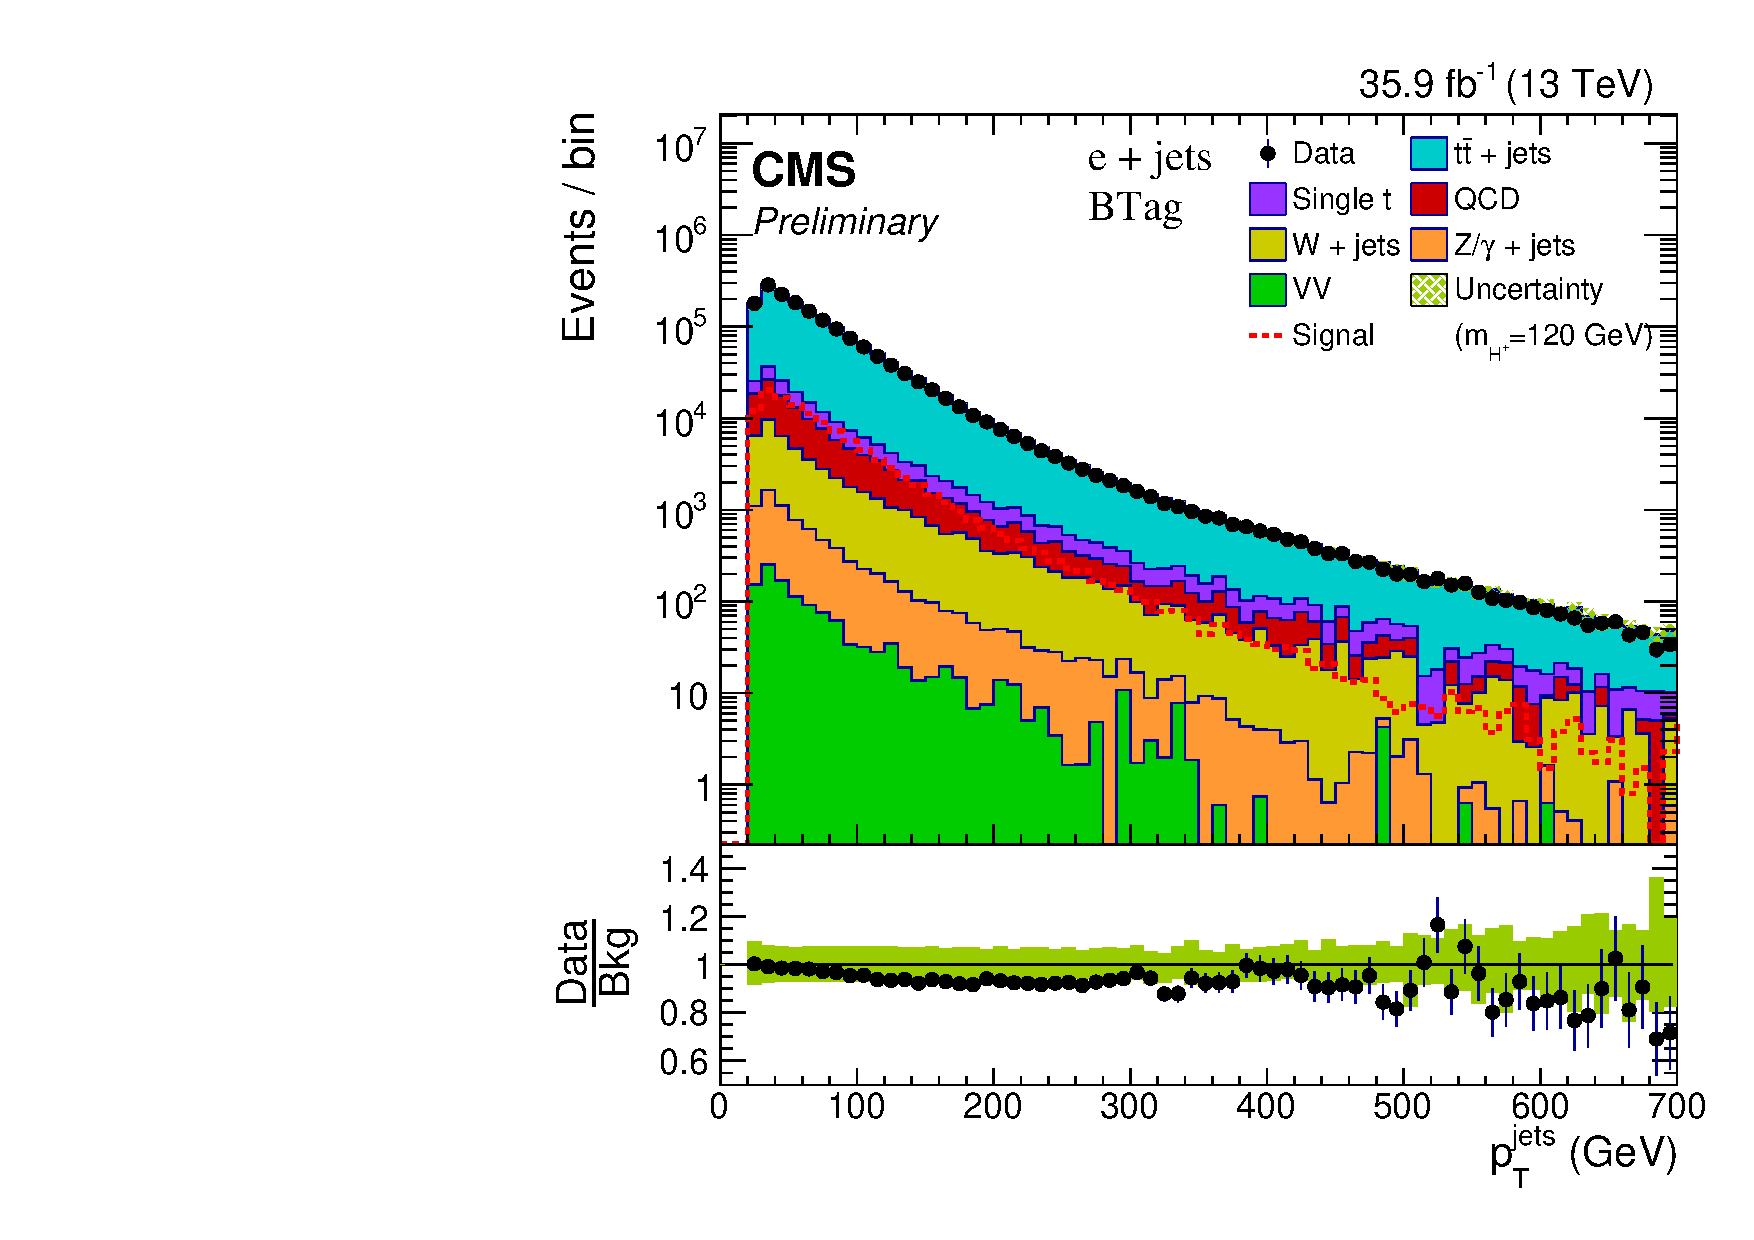
\includegraphics[width=0.40\linewidth]{Image/Electron/BTag/pt_jet_eleBTag.pdf}}
    \caption{Distribution of $\pt, \eta$ of reconstructed lepton and \pt of jets
        after \PQb jet selection as described in Section~\ref{s:secEvtSel}, 
    for \mujets and \ejets channel.}
    \label{fig:btagPlot1}
\end{figure}

%After BTagging: Eta_jets, N_jets, N_bjets
\begin{figure}
    \centering  
    \subfigure[$\eta$ of jets]{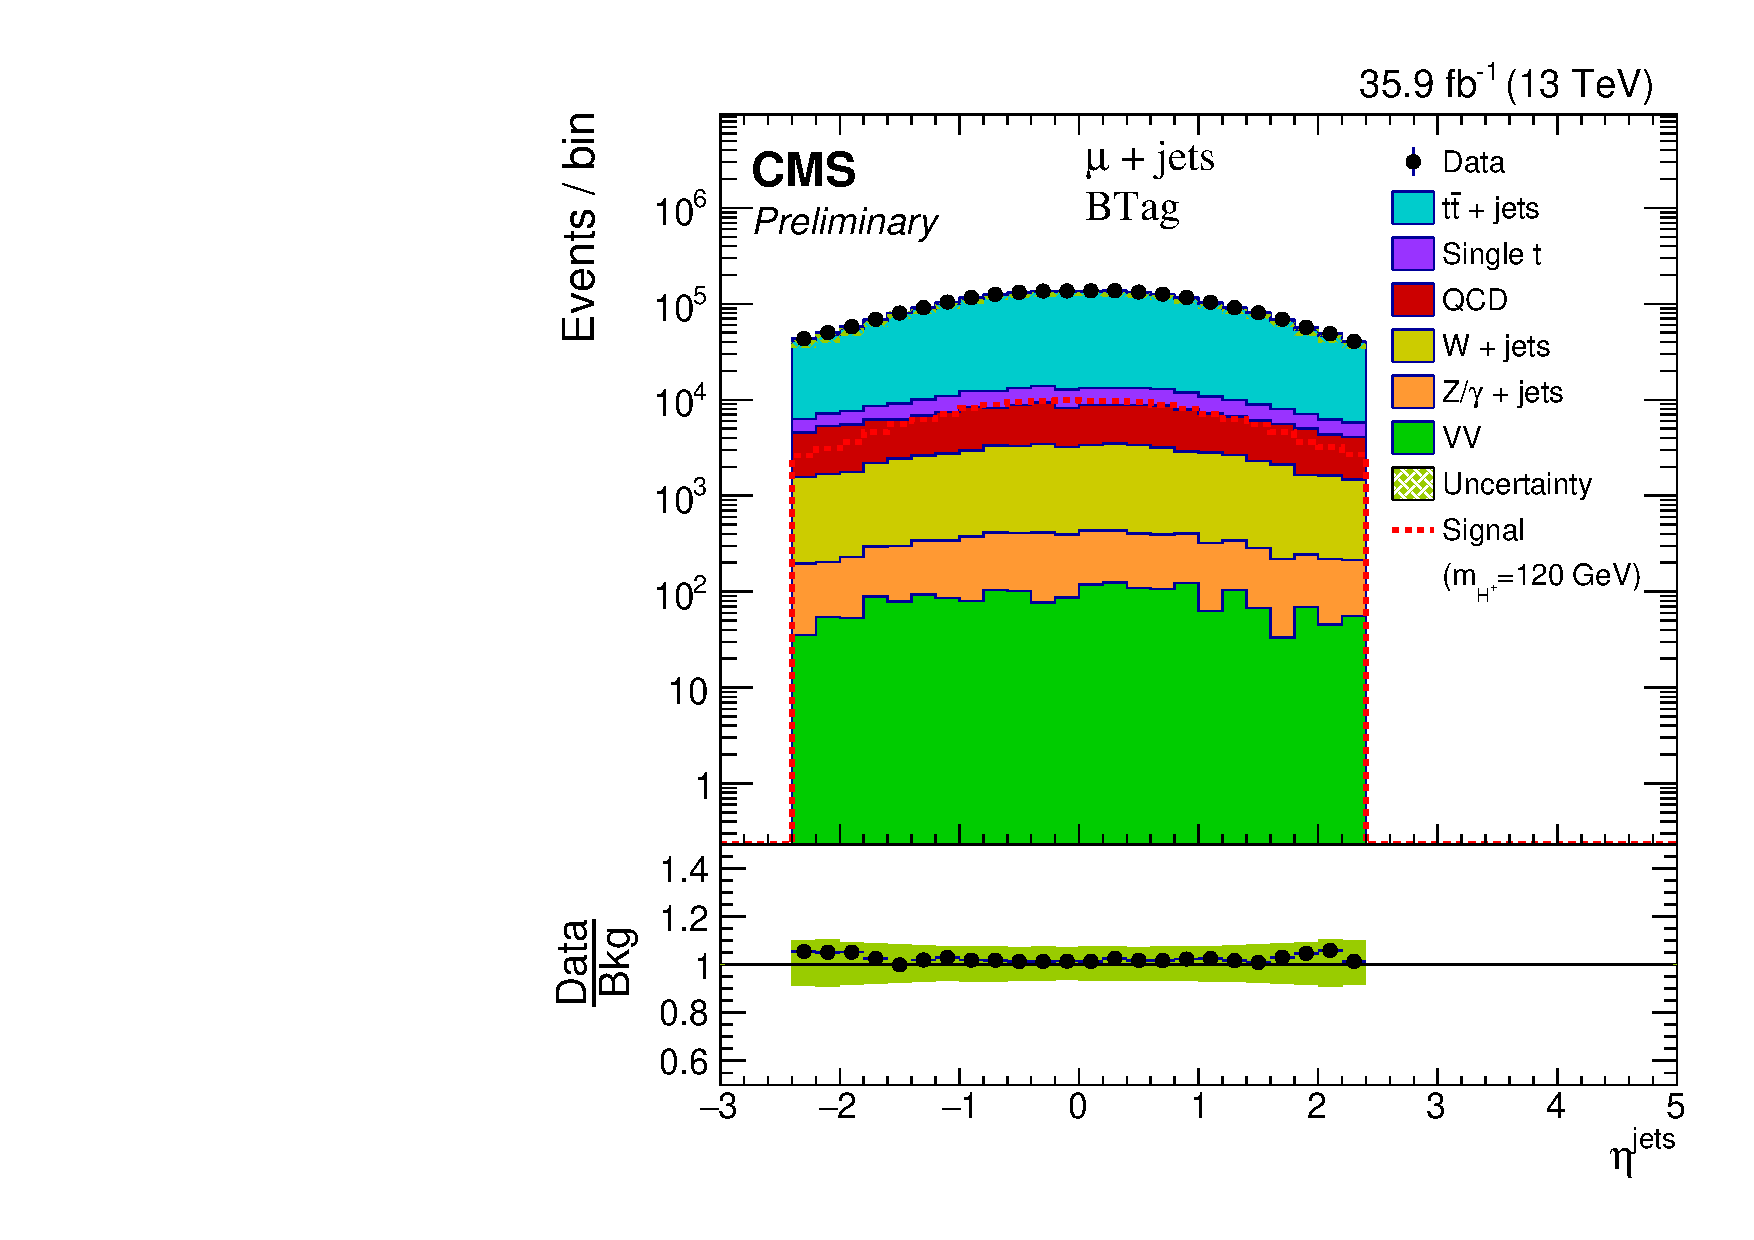
\includegraphics[width=0.40\linewidth]{Image/Muon/BTag/eta_jet_muBTag.pdf}}
    \subfigure[$\eta$ of jets]{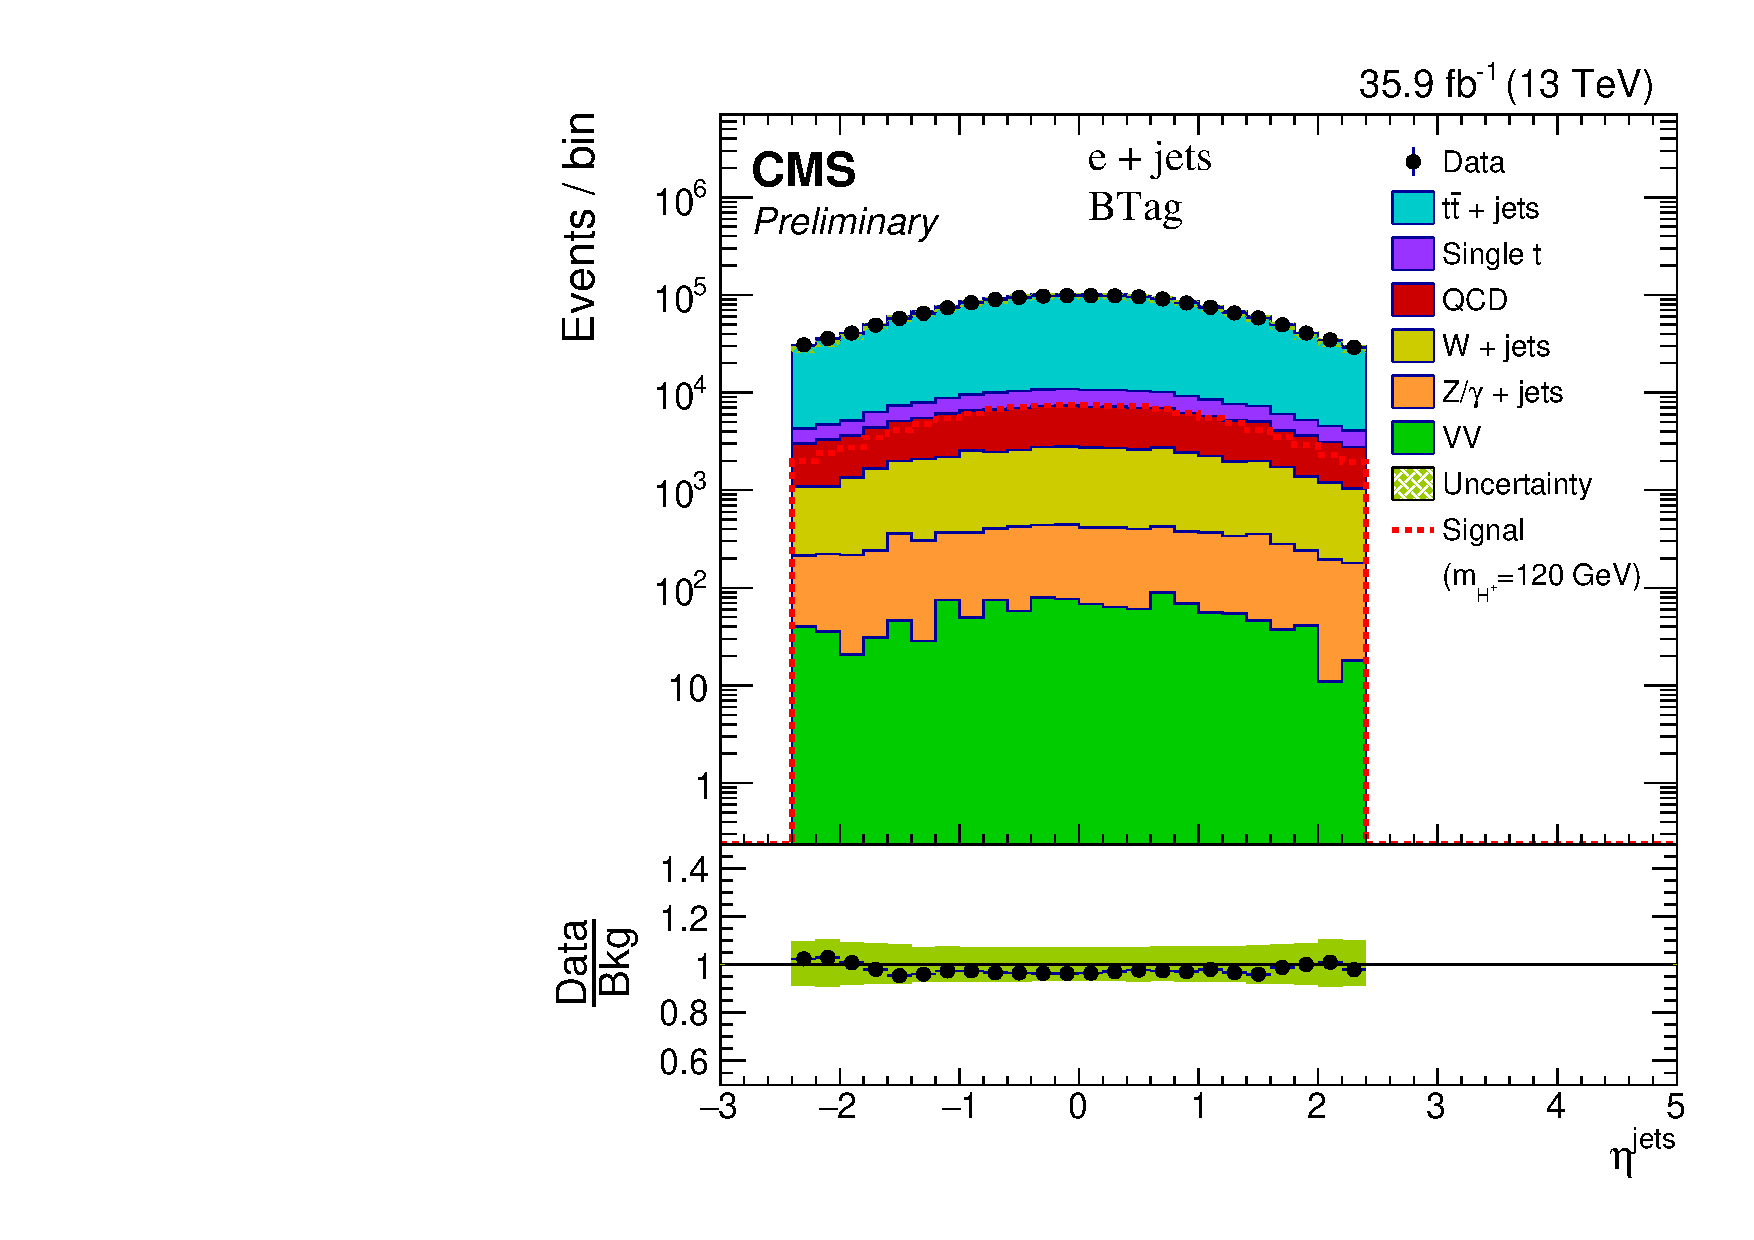
\includegraphics[width=0.40\linewidth]{Image/Electron/BTag/eta_jet_eleBTag.pdf}}
    \vfil
    \subfigure[jet multiplicity]{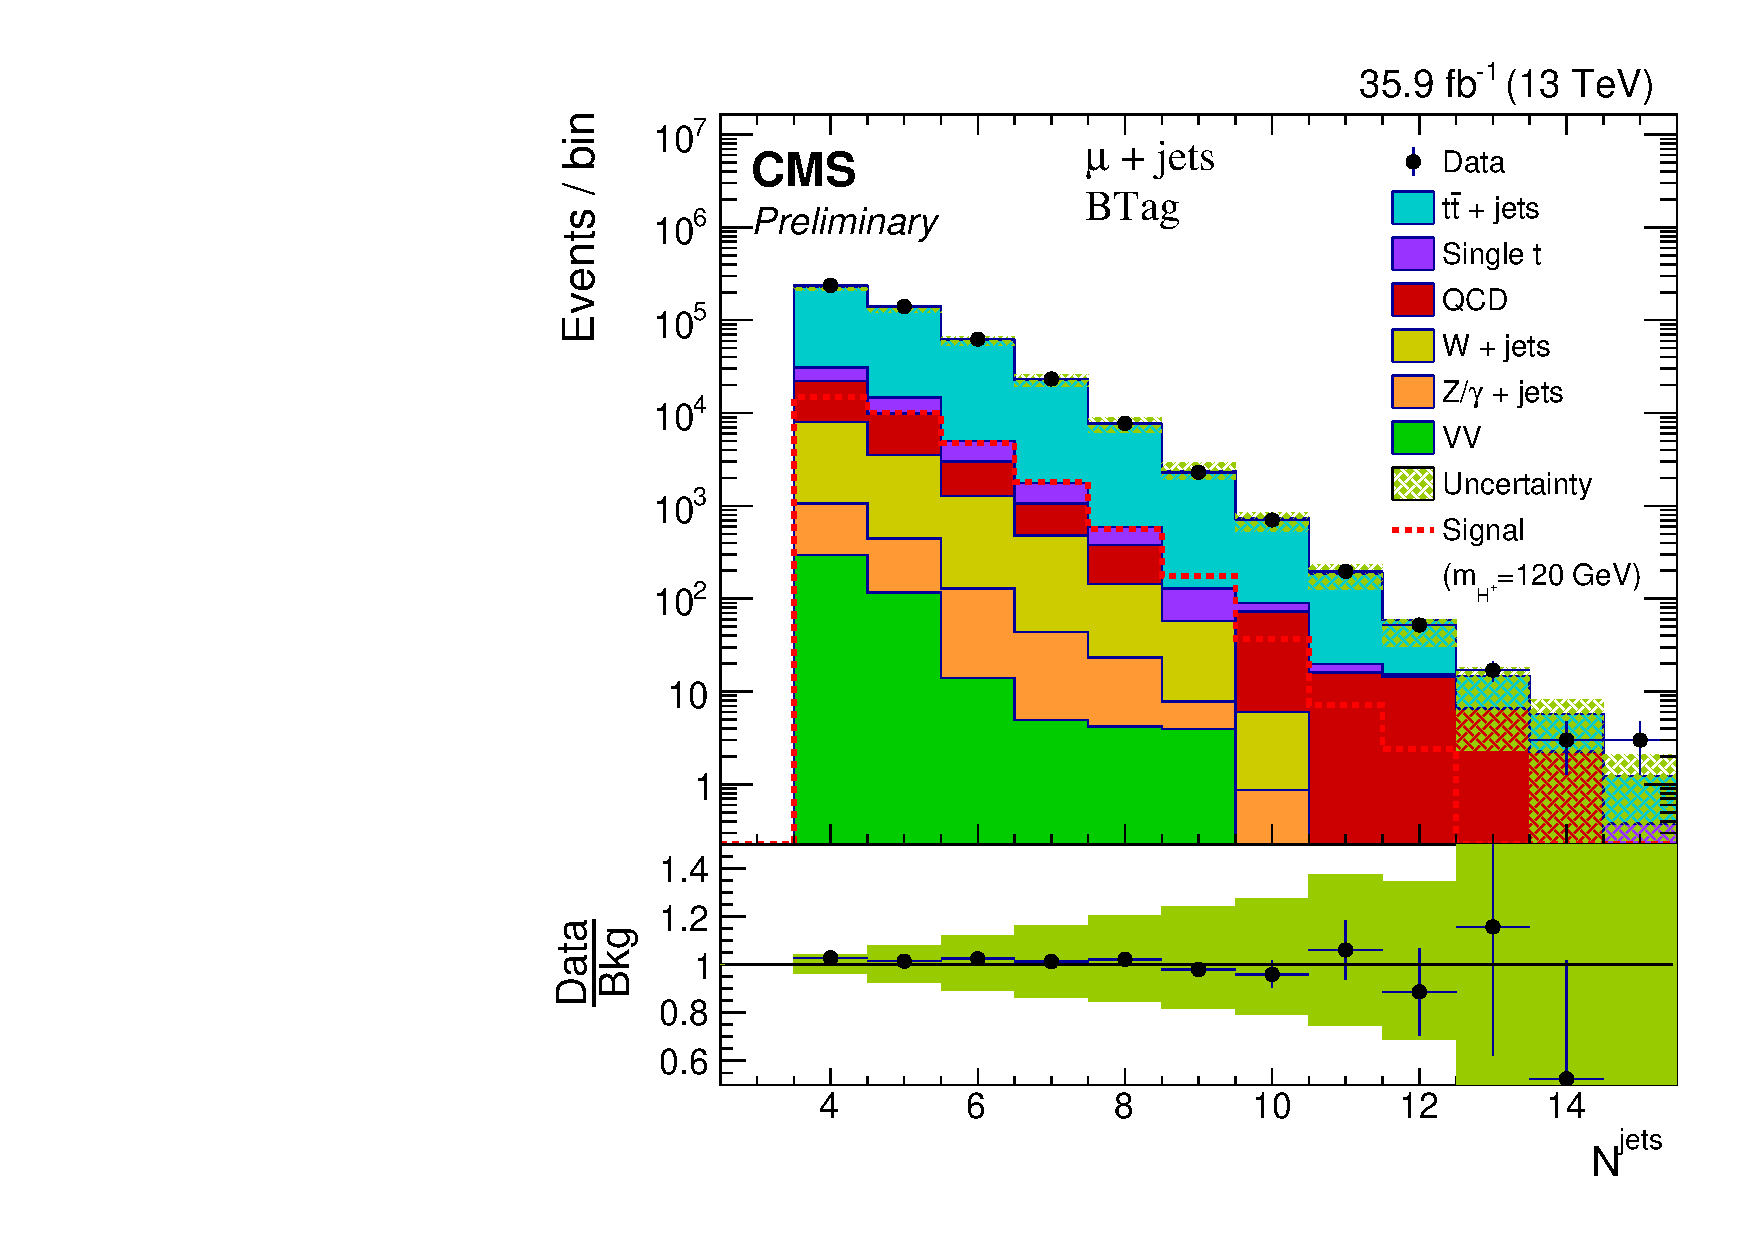
\includegraphics[width=0.40\linewidth]{Image/Muon/BTag/final_multi_jet_muBTag.pdf}}
    \subfigure[jet multiplicity]{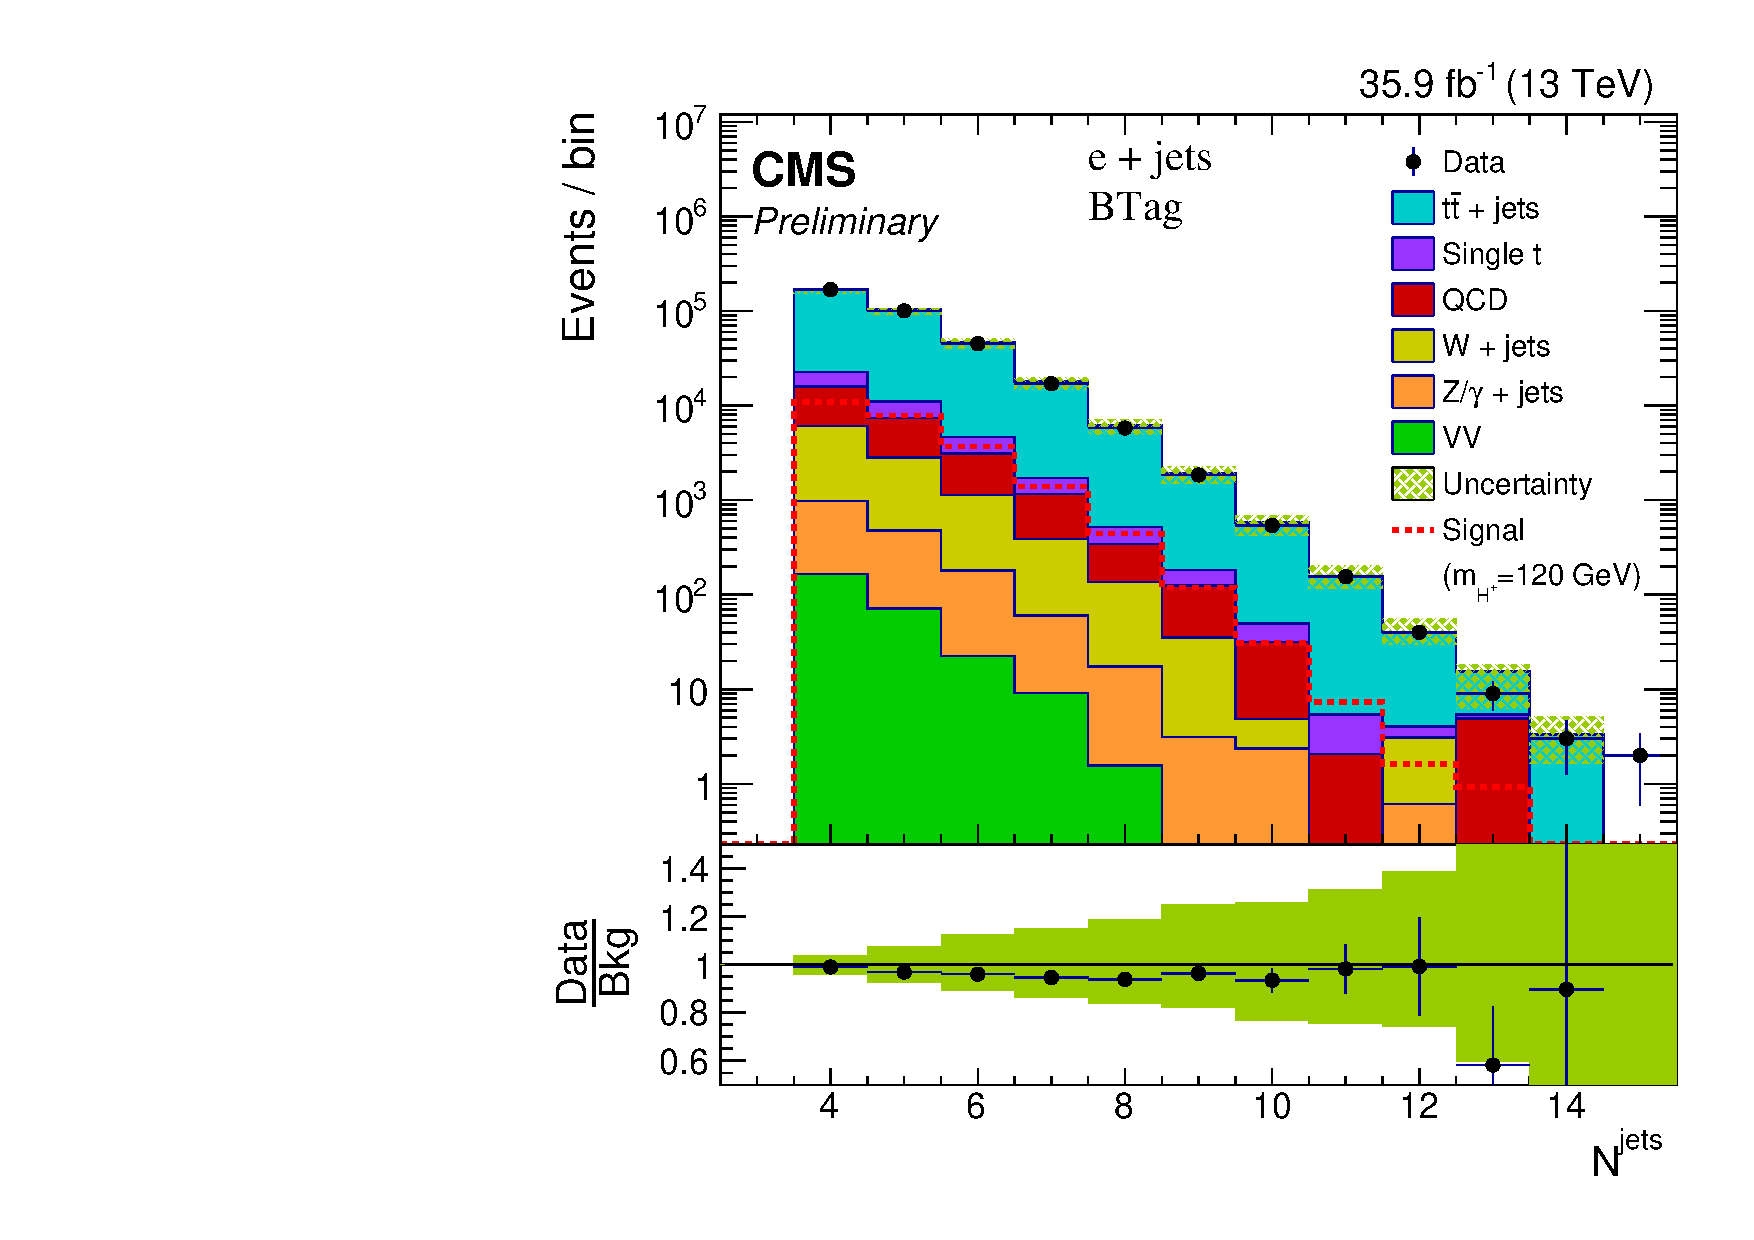
\includegraphics[width=0.40\linewidth]{Image/Electron/BTag/final_multi_jet_eleBTag.pdf}}
    \vfil
    \subfigure[\PQb jet multiplicity]{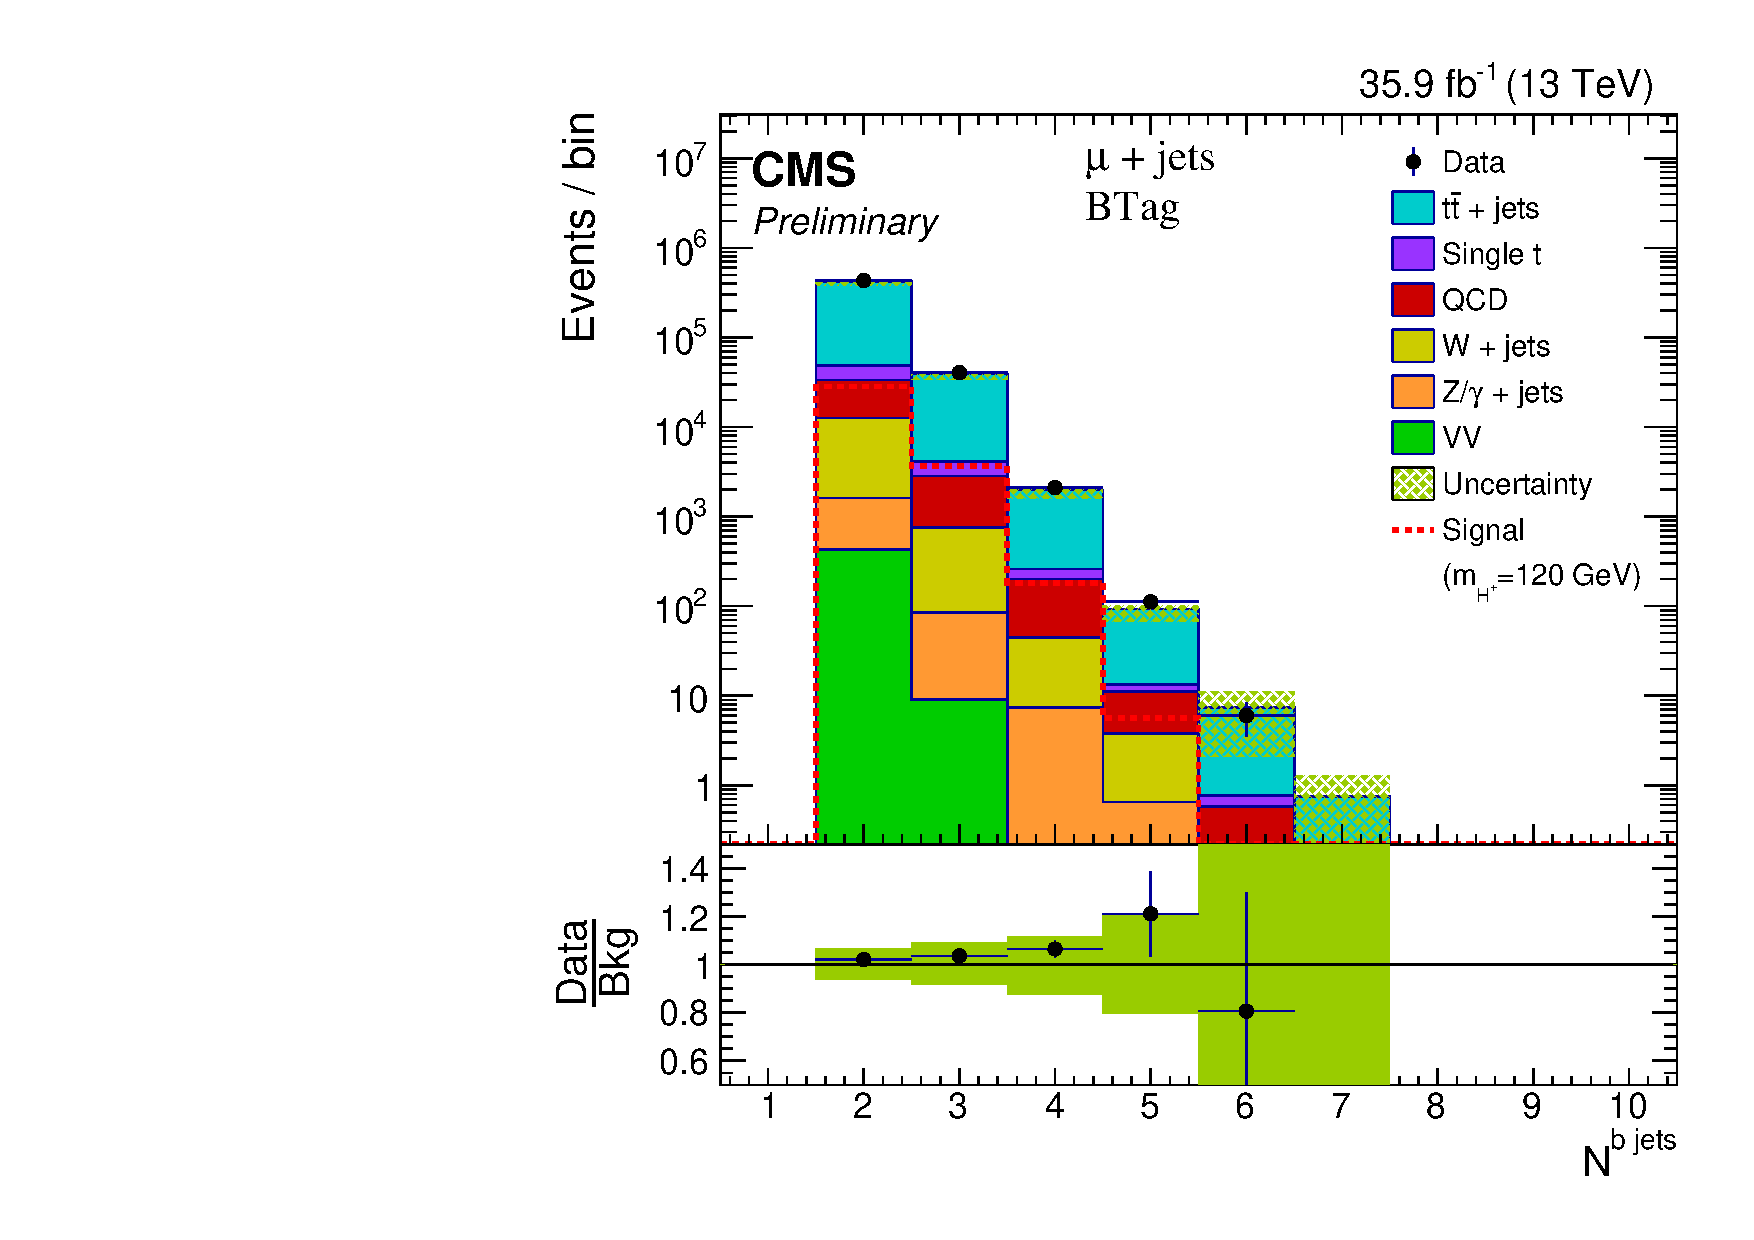
\includegraphics[width=0.40\linewidth]{Image/Muon/BTag/CSVL_count_muBTag.pdf}}
    \subfigure[\PQb jet multiplicity]{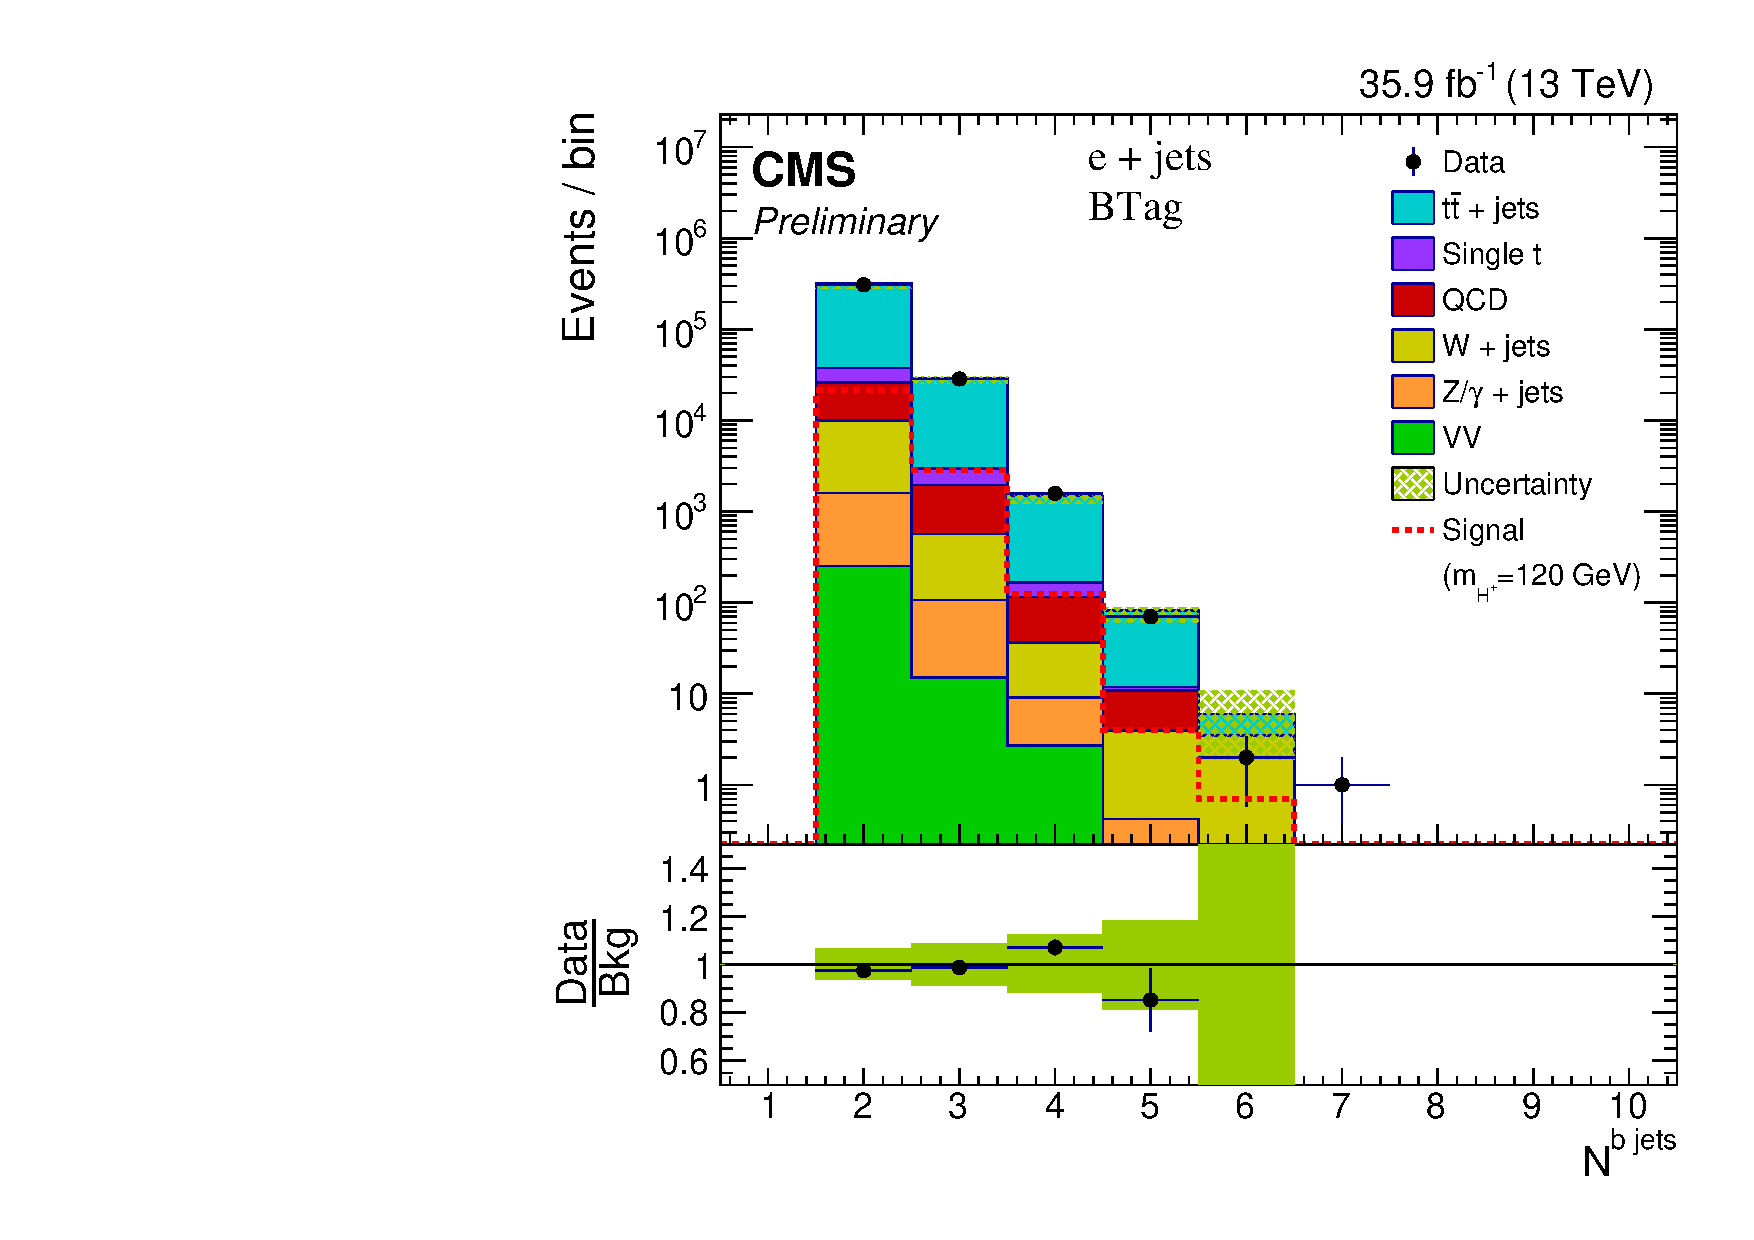
\includegraphics[width=0.40\linewidth]{Image/Electron/BTag/CSVL_count_eleBTag.pdf}}
    \caption{Distribution of reconstructed $\eta$ of jets, jet multiplicity, and 
        \PQb jet multiplicity after \PQb jet selection as described in 
        Section~\ref{s:secEvtSel}, for \mujets and \ejets channel.}
    \label{fig:btagPlot2}
\end{figure}

%After BTagging: \MET, MT 
\begin{figure}
    \centering  
    \subfigure[Missing transverse energy]{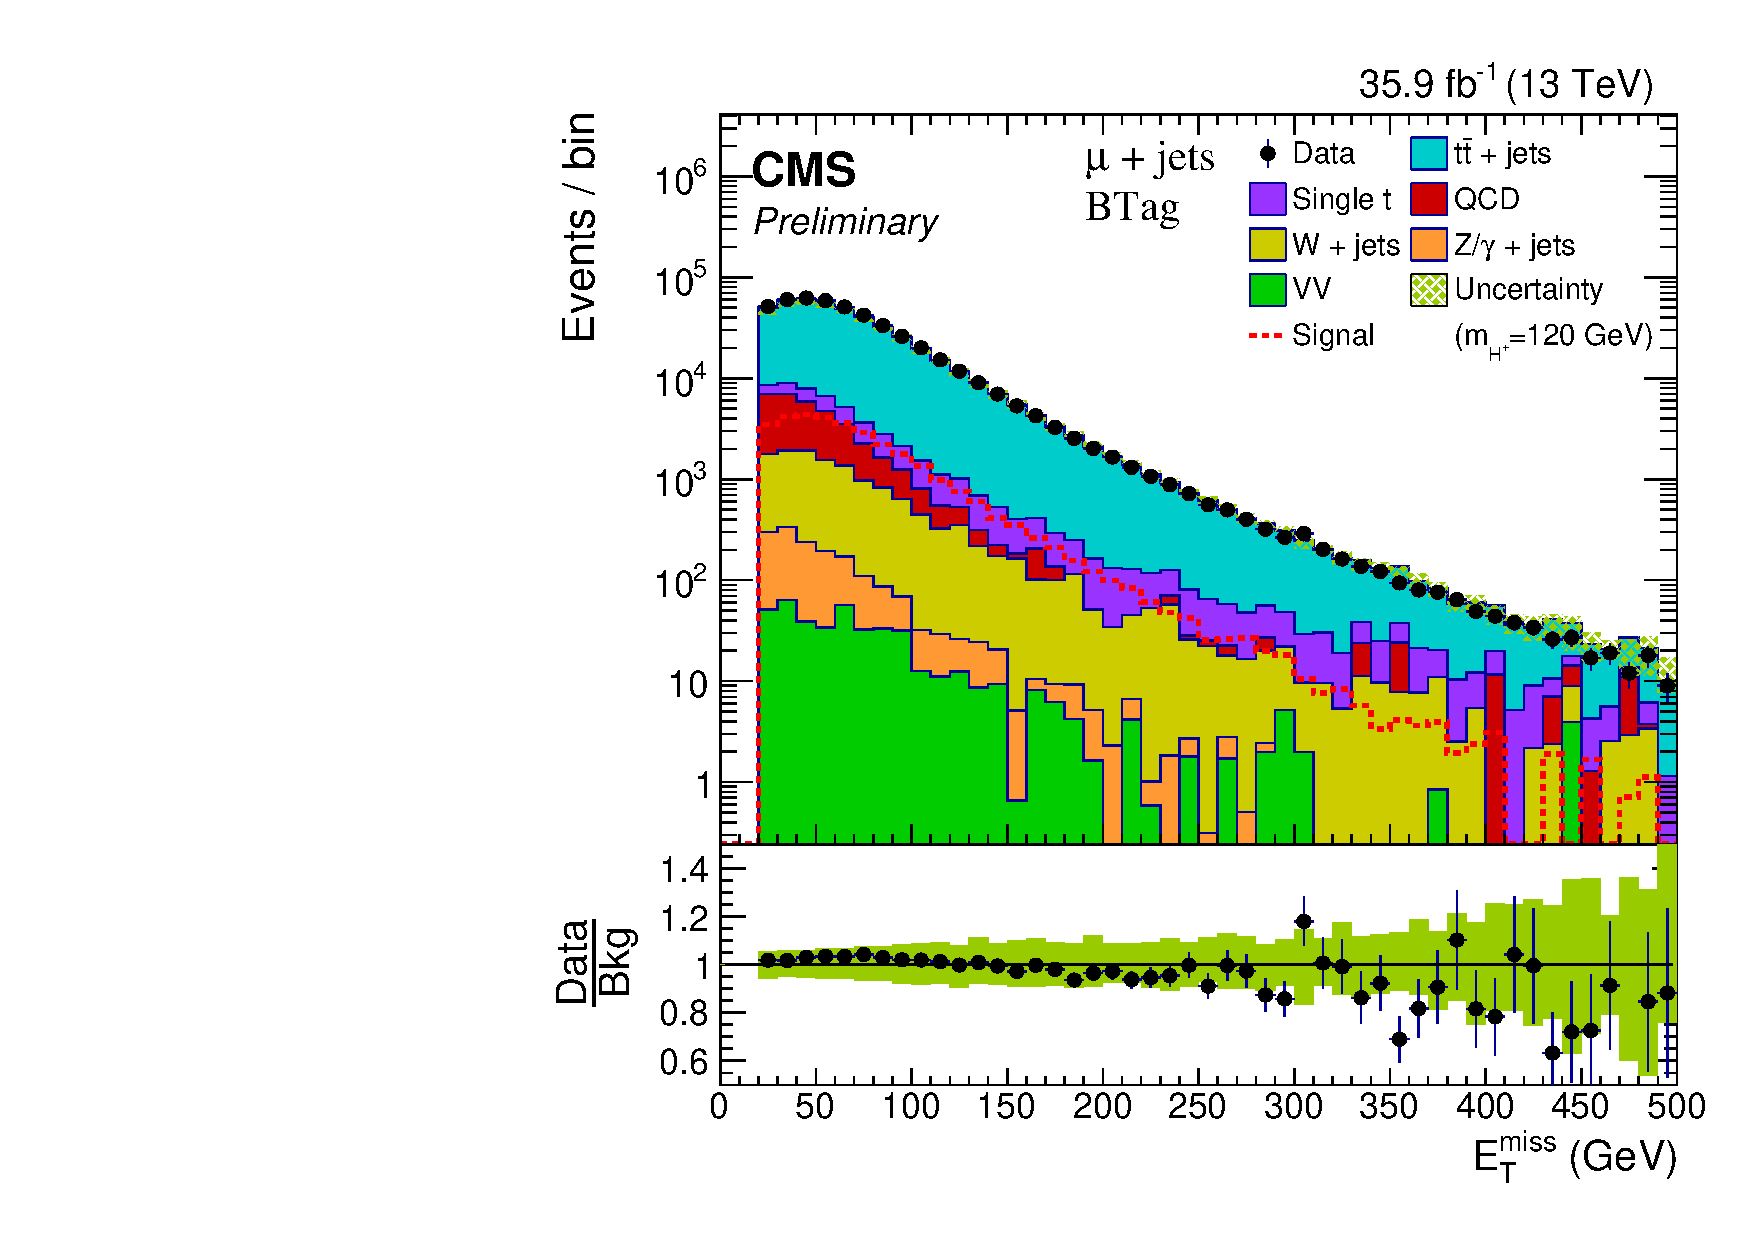
\includegraphics[width=0.45\linewidth]{Image/Muon/BTag/final_pt_met_muBTag.pdf}}
    \subfigure[Missing transverse energy]{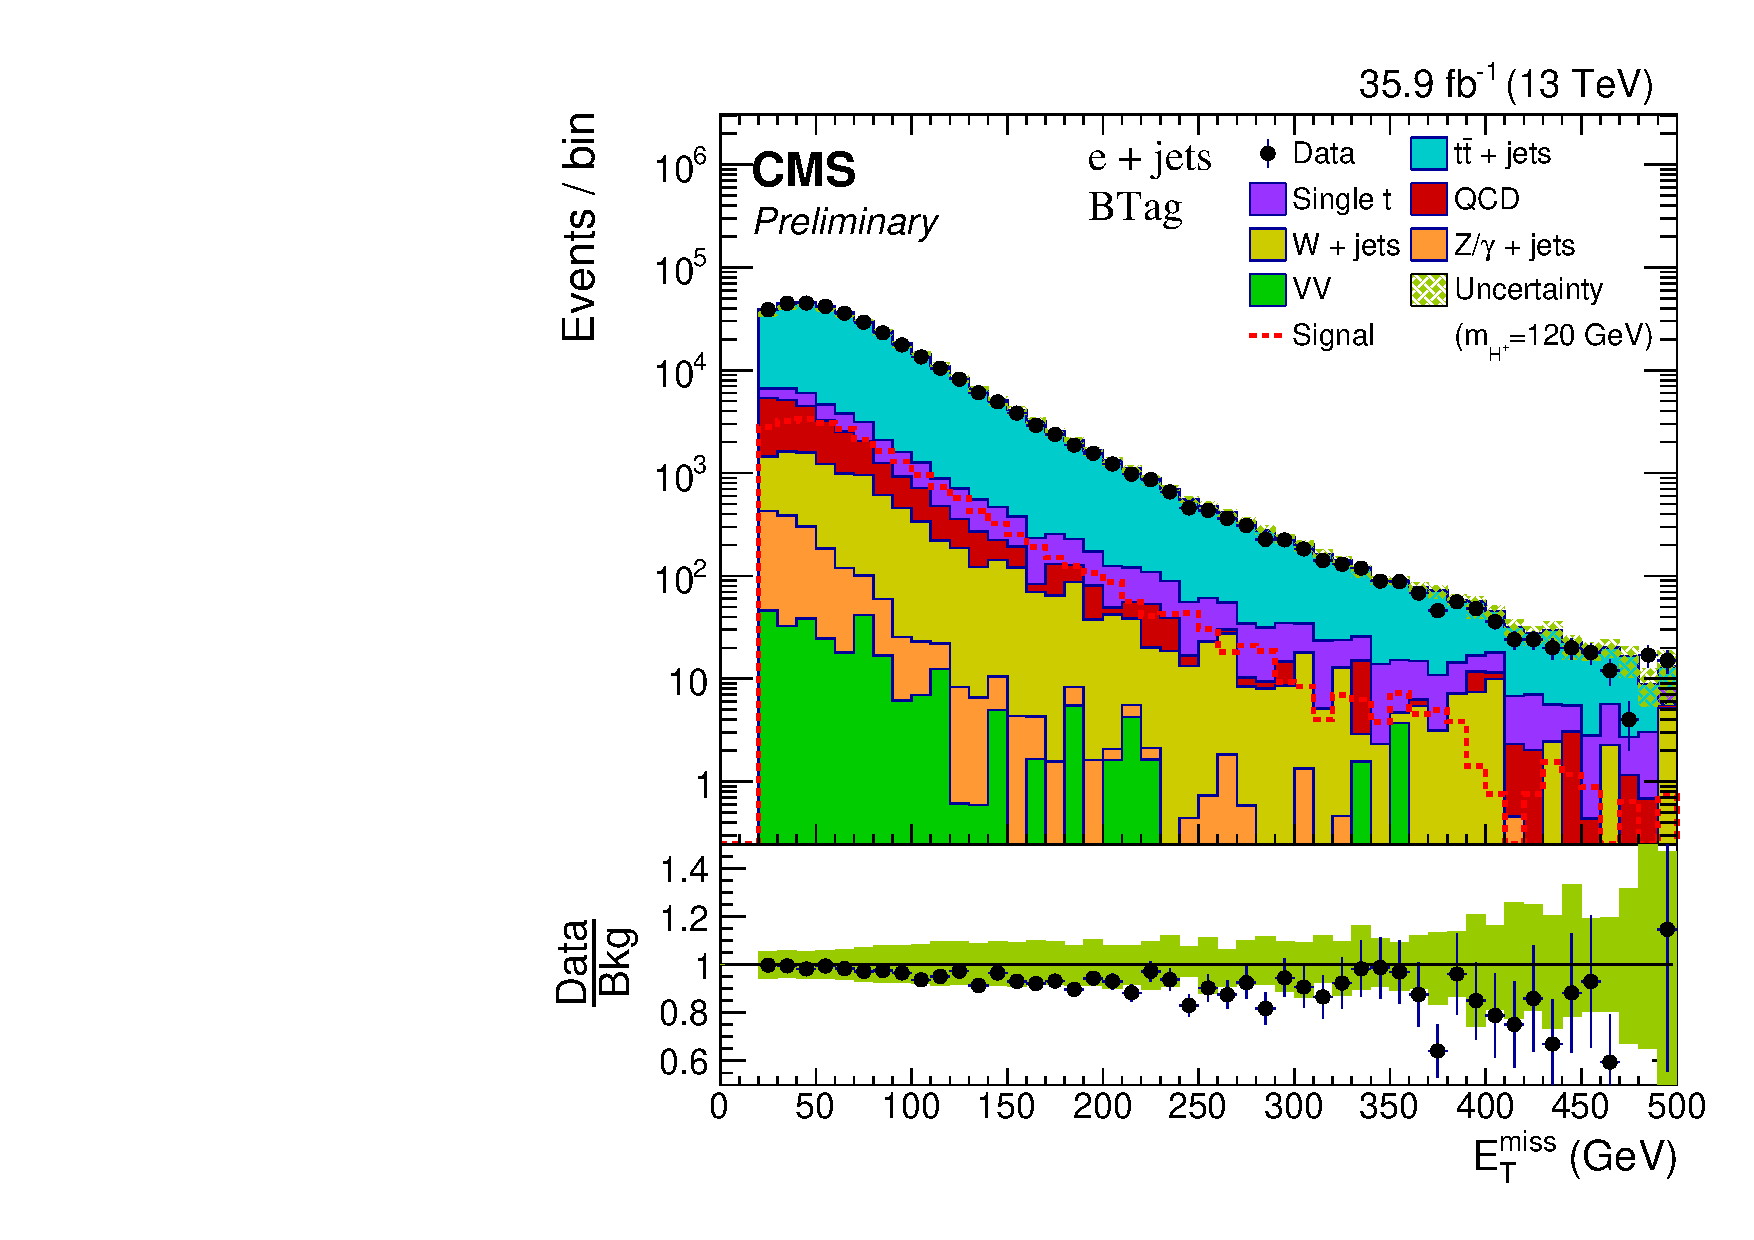
\includegraphics[width=0.45\linewidth]{Image/Electron/BTag/final_pt_met_eleBTag.pdf}}
    \vfil
    \subfigure[Transverse mass of \PW boson]{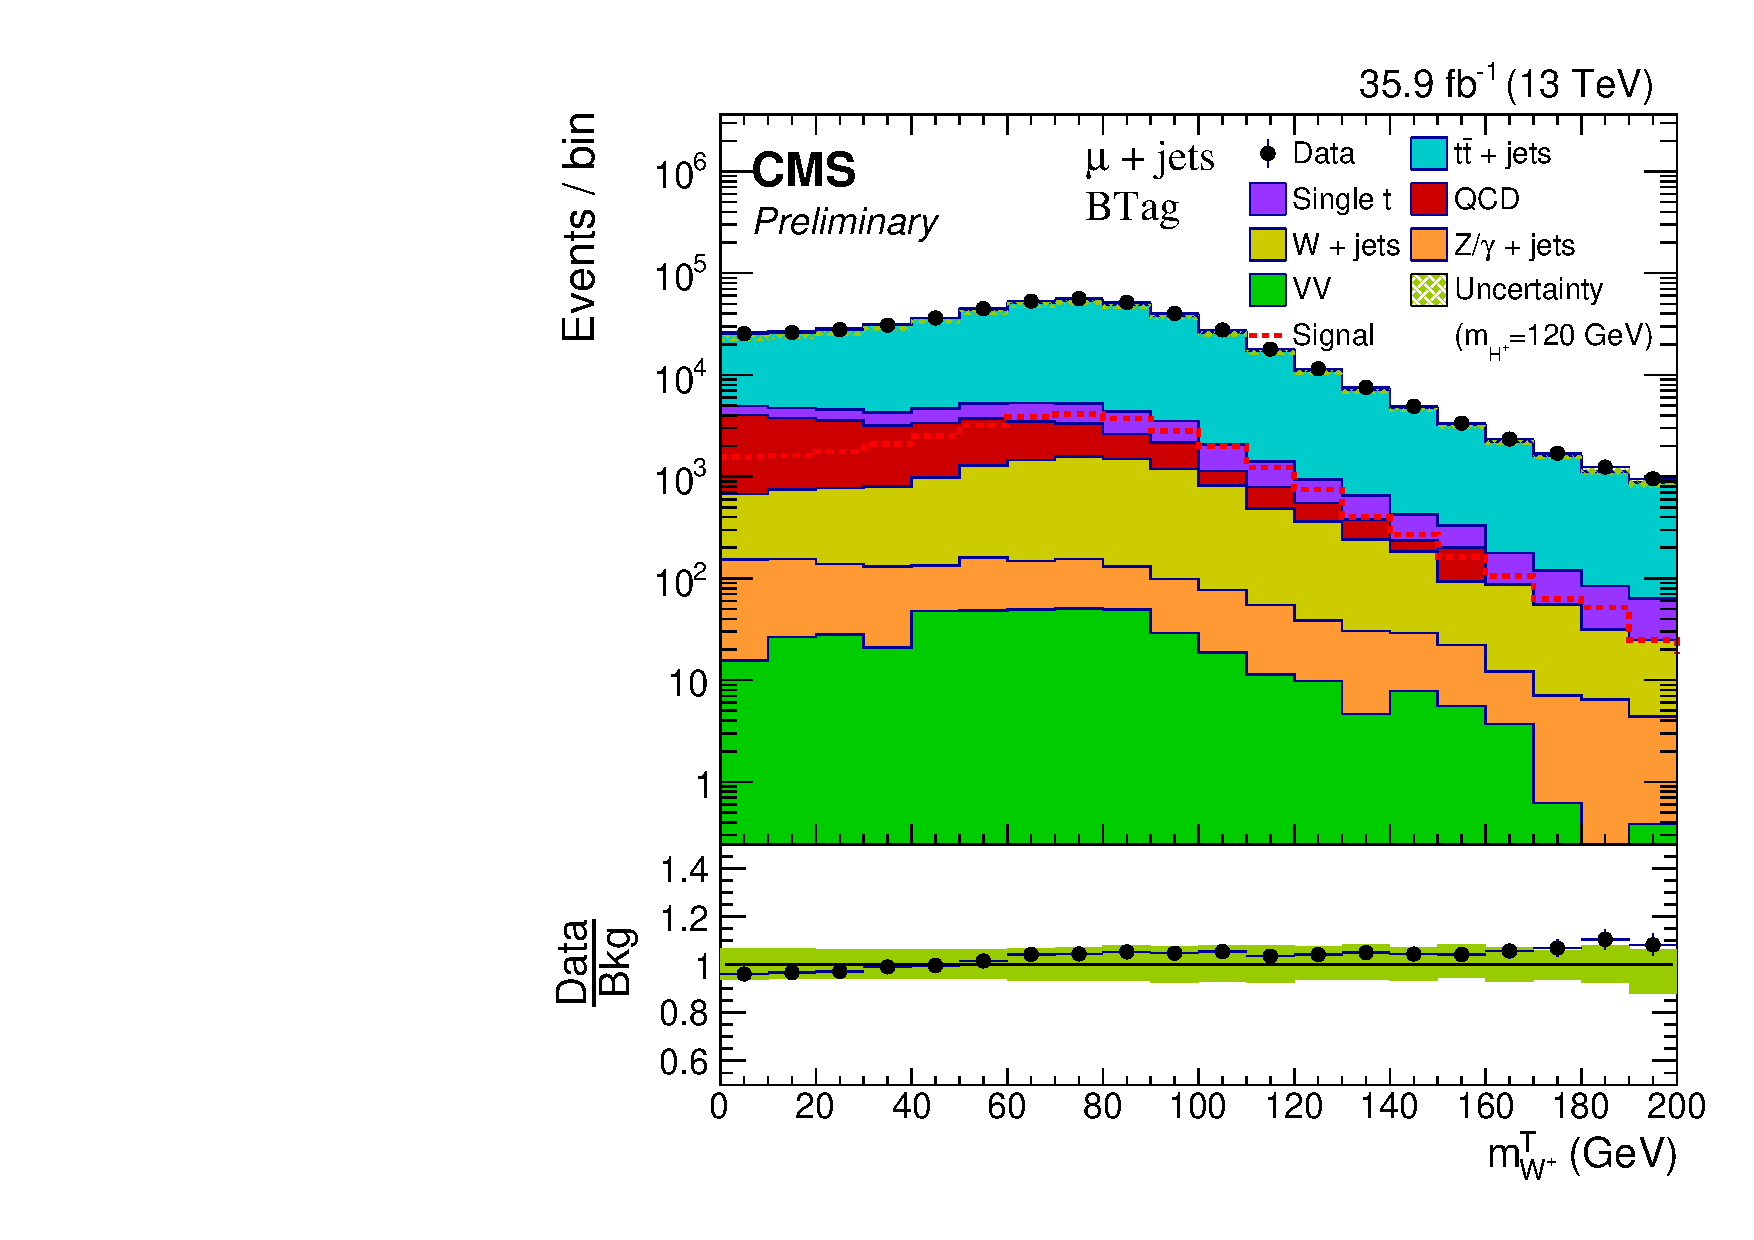
\includegraphics[width=0.45\linewidth]{Image/Muon/BTag/wmt_muBTag.pdf}}
    \subfigure[Transverse mass of \PW boson]{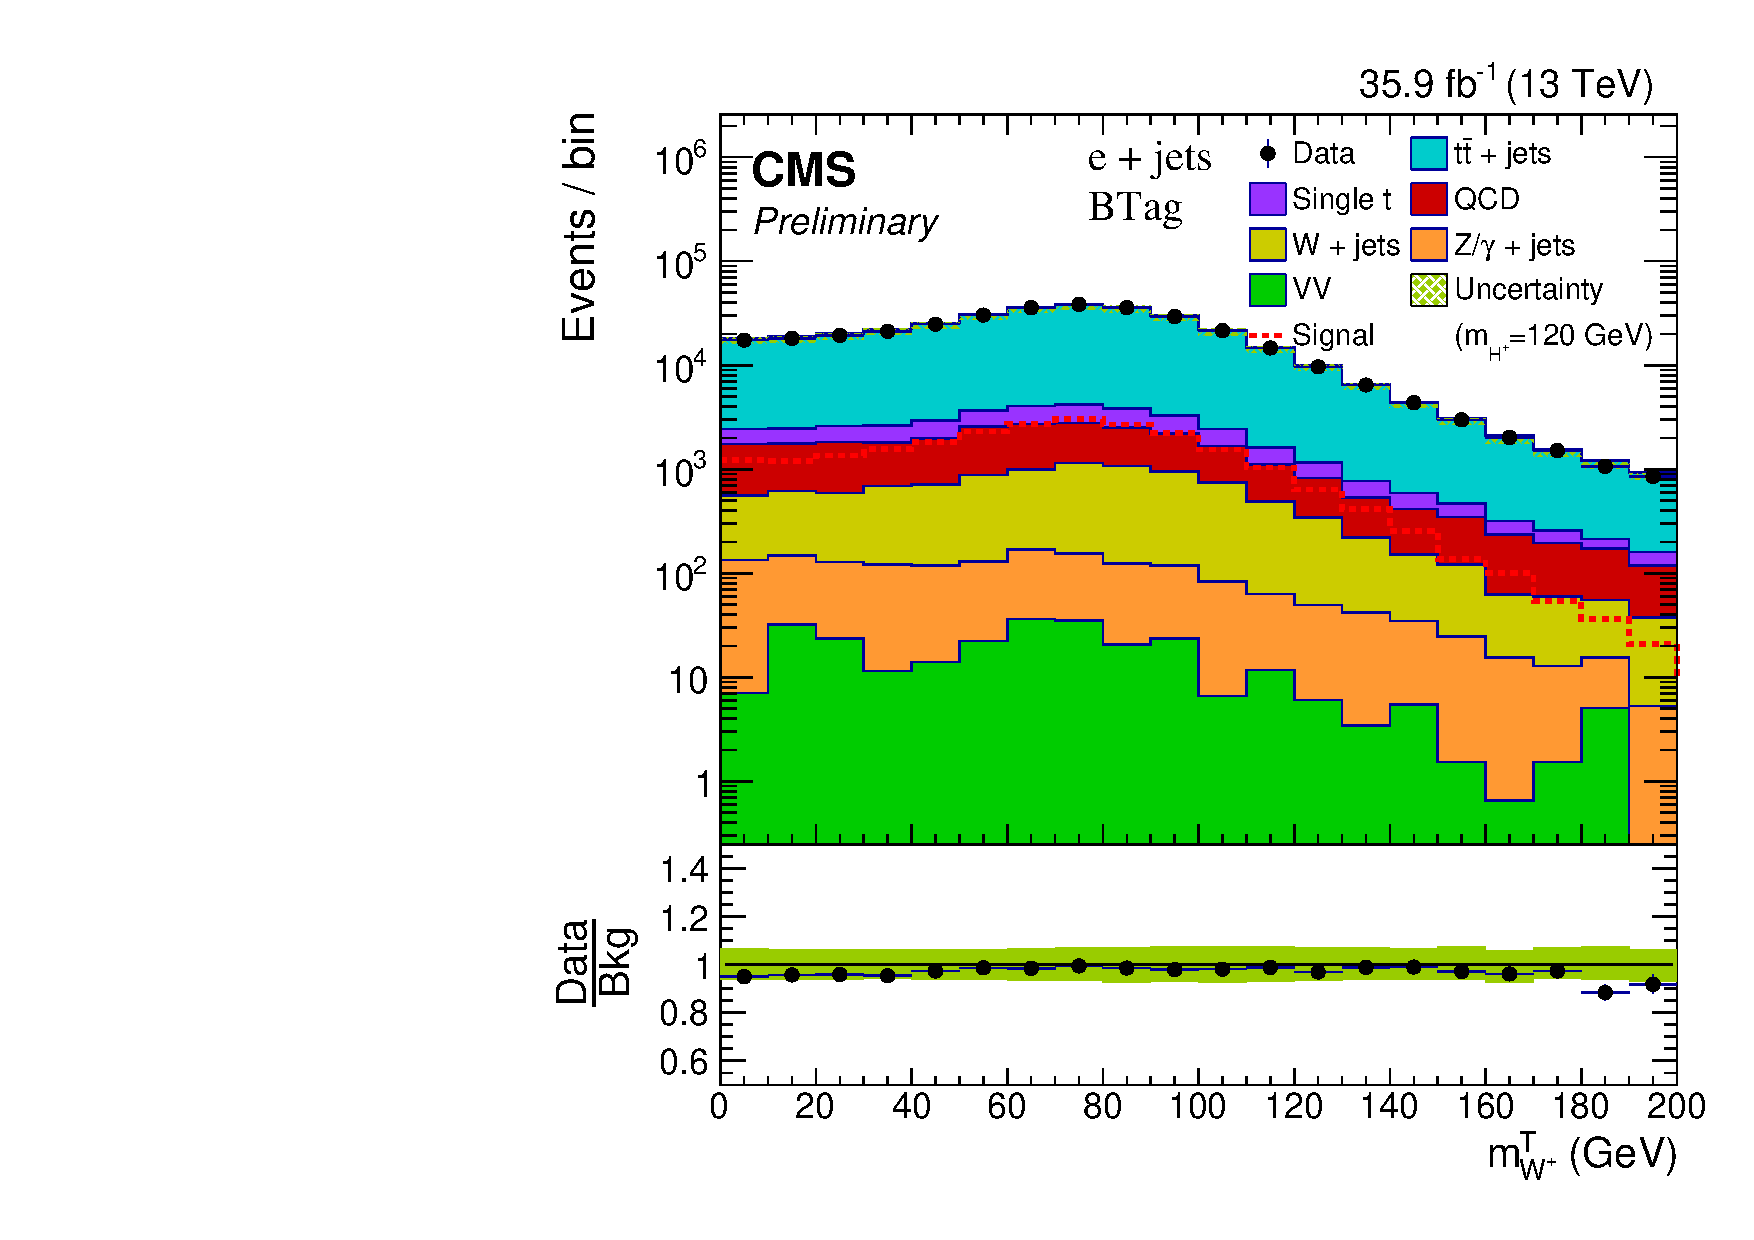
\includegraphics[width=0.45\linewidth]{Image/Electron/BTag/wmt_eleBTag.pdf}}
    \caption{Distribution of reconstructed $\MET$ and $m_{\PW^+}^{T}$ 
        (transverse mass of \PW boson decaying leptonically) after \PQb jet 
        selection as described in Section~\ref{s:secEvtSel}, for \mujets and 
    \ejets channel.}
    \label{fig:btagPlot3}
\end{figure}


